%                                                                 aa.dem
% AA vers. 9.1, LaTeX class for Astronomy & Astrophysics
% demonstration file
%                                                       (c) EDP Sciences
%-----------------------------------------------------------------------
%
%\documentclass[referee]{aa} % for a referee version
%\documentclass[onecolumn]{aa} % for a paper on 1 column  
%\documentclass[longauth]{aa} % for the long lists of affiliations 
%\documentclass[letter]{aa} % for the letters 
%\documentclass[bibyear]{aa} % if the references are not structured 
%                              according to the author-year natbib style

%
\documentclass{aa}  

%
\usepackage{graphicx}
%%%%%%%%%%%%%%%%%%%%%%%%%%%%%%%%%%%%%%%%
\usepackage{txfonts}
%%%%%%%%%%%%%%%%%%%%%%%%%%%%%%%%%%%%%%%%
%\usepackage[options]{hyperref}
% To add links in your PDF file, use the package "hyperref"
% with options according to your LaTeX or PDFLaTeX drivers.
\usepackage[colorlinks=true,citecolor=blue,linkcolor=blue]{hyperref}
% To add links in your PDF file, use the package "hyperref"
% with options according to your LaTeX or PDFLaTeX drivers.
%
\usepackage{natbib}
\bibpunct{(}{)}{;}{a}{}{,} % to follow the A&A style
%\usepackage{enumitem}
\usepackage{bm}
\usepackage{upgreek}
\usepackage[dvipsnames]{xcolor}
\usepackage{amsmath}    % Advanced maths commands
%\usepackage{amssymb}
%

\newcommand{\nlens}{15}

\begin{document} 


   \title{Investigating the relation between environment and internal structure of massive elliptical galaxies using strong lensing}

   \subtitle{}

   \author{BDLensing team
          \inst{1}
          \and
          C. Ptolemy\inst{2}\fnmsep\thanks{Just to show the usage
          of the elements in the author field}
          }

   \institute{Institute for Astronomy (IfA), University of Vienna,
              T\"urkenschanzstrasse 17, A-1180 Vienna\\
              \email{wuchterl@amok.ast.univie.ac.at}
         \and
             University of Alexandria, Department of Geography, ...\\
             \email{c.ptolemy@hipparch.uheaven.space}
             \thanks{The university of heaven temporarily does not
                     accept e-mails}
             }

   \date{Received ; accepted }

% \abstract{}{}{}{}{} 
% 5 {} token are mandatory
 
  \abstract
  % context heading (optional) 
  {}
  % aims heading (mandatory)
   {To investigate the relation between the internal structure of elliptical galaxies at $z \sim 0.5$ and their environment from a strong-gravitational lensing analysis. Particularly, to investigate two cases of correlation: between the (light and mass) centroid offset and the surrounding source density, and between the position-angle offset and the surrounding source density.}
   % methods heading (mandatory)
   {Using the publicly available software \textsc{lenstronomy}, we simulate images of a sample of 14 galaxy-galaxy lenses selected from the DESI survey. The process is based on the statistical method of Bayesian inference and utilizes the concepts of Particle Swarm Optimization (PSO) and Markov chain Monte Carlo (MCMC) sampling.}
   % results heading (mandatory)
   {Assuming $z \sim 0.5$, the mean centroid offset is within $200$ pc. The estimated biweight midcorrelation values for the two cases are $\sim$0.17 and $\sim$0.31, respectively.}
   % conclusions heading (optional), leave it empty if necessary 
   {The centroid offset is within the range predicted by the EAGLE simulation. Though the correlations are weaker than in some previous studies, the general trend is very similar. The lens model parameters embody information on dark matter haloes and can be utilized in the future. Furthermore, the estimated `external shear' parameters can be used in subsequent works based on \cite{Etherington23} and can help find flexible enough mass models for employment in future modelings.}

   \keywords{MCMC -PSO --
                gravitational lensing: strong
               }

   \maketitle
%
%-------------------------------------------------------------------

\section{Introduction}

Strong gravitational lensing is the phenomenon of forming multiple images from a background source due to the gravitational bending of light path by a massive foreground deflector, such as a galaxy, galaxy group, or cluster. As a result, strong lensing systems are powerful probes of the mass distribution of the foreground deflector \citep[see][for a review on strong lensing by galaxies]{Shajib22}.

Whereas the observed light traces the stars in a lensing galaxy, strong lensing traces the total matter distribution, including dark and baryonic components. As a result, strong lensing can be used to study the relative alignment between dark matter and stars. Any detected offset between these two components can indicate self-interaction in the dark matter particles \citep{Harvey14, Kahlhoefer14, Robertson17}. In the $\Lambda$ cold dark matter ($\Lambda$CDM) cosmology -- the current paradigm to describe our Universe -- the EAGLE simulation predicts no significant offset $\sim$200 pc, regardless of the galaxy being a field galaxy or a cluster member \citep{Schaller15}. Although a recent merger can lead to an offset between the dark matter and stars, these systems are statistically very rare \citep{Schaller15}. On the observational front, only one system has been observed with an offset much larger than this prediction ($1.72\pm 0.42$ kpc), where the deflector consists of two merging galaxies  \citep[][]{Shu16}. %Although there was an initial report of a similar offset for a cluster-member galaxy in Abell 3827 \citep{Williams11, Massey15}, the offset was ruled out with more data \citep{Massey18}.
\citet{Shajib19} find a root-mean-square (RMS) offset in a sample of 15 strong lenses to be 0\farcs04 (i.e., $\sim$200 pc at z$\sim$0.5) excluding three outliers, one of which has two comparable-mass deflectors potentially residing in the same parent halo. Similarly, \citet{Shajib21} constrained a 68 percent upper limit of 218$\pm$19 pc from a sample of 23 galaxy--galaxy lenses.

The misalignment between the mass and light distributions can also be traced using the position angles of the major axes of the elliptical galaxies, which are the most common type of deflectors at the galaxy scale. Previous studies mostly found tight alignment within $\sim$10$\degr$ \citep{Keeton98b, Kochanek02, Treu09, Gavazzi12, Sluse12, Bruderer16, Shajib19, Shajib21}, with higher misalignments are accompanied by large ``external'' shear magnitude, although the vice versa is not necessary. The accompaniment of a large ``external'' shear with a large misalignment can be interpreted as systems in a crowded environment that are not yet dynamically relaxed, as they can have stellar orbits misaligned with the underlying dark matter distribution. Simulations found highly misaligned orbits in isolated systems to be unstable and rare \citep{Heiligman79, Martinet88, Adams07, Debattista15}. However, this interpretation treats ``external'' shear as originating purely from nearby line-of-sight galaxies external to the central deflector. Interestingly, \citet{Etherington23} suggested that this ``external'' shear is not purely of external origin and can arise from the inadequacy of the mass model for lensing galaxy in capturing all of its angular complexity \citep[for example, boxy/discyness, ellipticity gradient, isophotal twists;][]{VandeVyvere22, VandeVyvere22b}. This suggestion from \citet{Etherington23} makes the explanation of high misalignment as stemming from interaction with a crowded environment less favorable.

In this paper, we investigate the alignment between the mass and light using a sample of \nlens\  galaxies. We present power-law mass models of these systems based on \textit{Hubble Space Telescope} (\textit{HST}) imaging data. Using our lens models, we perform two experiments. First, we check if there is a difference in the mass and light offset between isolated and non-isolated galaxies and test the prediction of no difference from the EAGLE simulation. Second, we investigate if the misalignment between light and mass major axes directly correlates with the local galaxy density. This second experiment more directly tests the hypothesis that galaxies with stellar orbits misaligned with dark matter live in crowded environments without adopting the ``external'' shear as a measure of a crowded environment.

This paper is organized as follows. In Section \ref{sec:data}, we describe the \textit{HST} data we model. Then in Section \ref{sec:modeling_method}, we describe our lens modelling method and our lens sample. We present our results in Section \ref{sec:result}. Finally, we discuss our result and conclude the paper in Section \ref{sec:discussion}. Throughout the paper, we adopt a flat $\Lambda$CDM cosmology as the fiducial cosmology with $H_0= 70$ km s$^{-1}$ Mpc$^{-1}$ and $\Omega_{\rm m} = 0.3$.

\section{Data} \label{sec:data}

Our sample comprises \nlens\ strong lensing systems (illustrated in Fig. \ref{fig:montage}). These systems were discovered as lens candidates in the Dark Energy Spectroscopic Instrument (DESI) Legacy Imaging Surveys, Data Release 7, using a deep neural network and then confirmed using the follow-up \textit{HST} imaging from the program SNAP-15867 (PI: Huang) analyzed in this paper. % Each system in our sample has multiple lensed images. In this section, we first describe the high-resolution imaging data obtained through HST. We then provide a brief overview of the lens systems in the sample.
% \subsection{\textit{HST} imaging} \label{sec:hst_imaging}
The \textit{HST} imaging was obtained using the Wide Field Camera 3 (WFC3) in the infrared (IR) channel using the F140W filter. The wide F140W filter covers the gap between the J and H bands that is inaccessible from the ground. 

We produced science-quality reduced images by combining multiple exposures using the \textsc{astrodrizzle} software package \citep{Avila15}.\footnote{The data reduction procedure followed the \textsc{jupyter} notebooks from this GitHub repository: \url{https://github.com/ajshajib/hst-lens}.} The drizzling process with \textsc{astrodrizzle} removed cosmic rays from the single exposure images. We chose 0\farcs8 as the pixel scale of the final image after drizzling. %, and 0.08 arcsec for WFC3 IR.
The final images were rotated through the drizzling process so that the North and East directions align with the vertical and horizontal directions, respectively. We used the \textsc{Python} package \textsc{PhotUtils} to estimate the mean background light and subtracted it from each image. The total noise per pixel was estimated by summing in quadrature the background root-mean-square level with the Poisson noise corresponding to the background-subtracted-flux in each pixel.


% example https://arxiv.org/pdf/2008.11724.pdf and https://arxiv.org/pdf/1807.09278.pdf




\section{Lens modeling} \label{sec:modeling_method}

To model the lenses, we used the lens modeling software \textsc{lenstronomy}, publicly available on GitHub\footnote{\url{https://github.com/lenstronomy}} \citep{Birrer15, Birrer18}.

\subsection{Lens model ingredients}
We need to pick baseline models for the lens mass and light to create a method that works well for many lensing systems of different sizes and shapes. These models can be adjusted case by case to fit the specific goals of the investigator. The idea is to make sure the models fit the data nicely while being flexible enough for a wide range of lens systems.\\

First, we commence with fundamental models for the lens mass, light, and source-light distribution, as delineated in Sections \ref{sec:mass_profile} and \ref{sec:light_profile}. Subsequently, we employ a Particle Swarm Optimization (PSO) routine in \textsc{Lenstronomy} to ascertain the optimal fit. Following this, we assess the model's fidelity to the data. Should it prove inadequate, we incrementally incorporate additional intricacies into the model. This may entail integrating more mass or light specifications to accommodate supplementary elements such as satellites, intricate structures adjacent to the Einstein ring, or additional lensed sources.\\

We also adjust the data, adding or removing bits using masks to make the modeling easier. We run the PSO routine again after each change until the chosen mass and light models give a good fit. Next, we figure out the likelihood of different model parameters using a Markov Chain Monte Carlo (MCMC) routine. For both modeling processes, we required an approximate $\chi^2\sim 1$ to fit our data which is a satisfactory value that covers most of our unique models. The PSO and MCMC routines in \textsc{Lenstronomy} use a package called \textsc{cosmoHammer}, which includes \textsc{emcee}, a smart way to explore different possibilities in the model. This approach helps us model lens systems in a detailed and effective manner.


\subsubsection{Mass profile} \label{sec:mass_profile}
% EPL, external shear 
% example https://arxiv.org/pdf/1807.09278.pdf
\paragraph{\textbf{EPL:}}
 The Elliptical Power Law mass profile is given by, 

$$
\kappa\left(x, y\right)=\frac{3-\gamma}{2}\left(\frac{\theta_{\mathrm{E}}}{\sqrt{q x^2+y^2 / q}}\right)^{\gamma-1}.
$$

The Elliptical Power Law (EPL) mass profile represents a specific form of the mass distribution used in gravitational lensing studies. It describes the convergence (\(\kappa\)) in terms of the coordinates \(x\) and \(y\) in an elliptical system, where \(x\) and \(y\) represent the Cartesian coordinates on the lens plane, and \(\theta_{\mathrm{E}}\) is the Einstein radius. The parameter \(q\) denotes the axis ratio of the ellipse, representing the elongation or flattening of the mass distribution.\\

\paragraph{\textbf{SIE:}} Singular Isothermal Ellipsoid (SIE) is given by,

$$
\kappa\left(x, y\right)=\frac{1}{2}\left(\frac{\theta_{\mathrm{E}}}{\sqrt{q x^2+y^2 / q}}\right)
$$

The factor $\frac{1}{2}$ is introduced to scale the convergence appropriately for the SIE model. We used this profile for the fit of the neighboring satellite galaxies.
\\

\paragraph{\textbf{Shear:}} Shear is a measure of the differential stretching or distortion of the images of background sources due to the gravitational lensing effect. It quantifies how much the shapes of background objects are elongated or deformed by the gravitational field of the lensing mass.\\


The pseudo-vector $\bm{\gamma}$=$(\gamma_1, \gamma_2)$ on the lens plane, whose components are
%

\begin{equation}
    \begin{aligned}
        & \gamma_1(\bm{x})=\frac{1}{2}\left(\Psi_{11}-\Psi_{22}\right) \\
        & \gamma_2(\bm{x})=\Psi_{12}=\Psi_{21},
    \end{aligned}
\end{equation}

%
This is called the shear. The eigenvalues of the shear matrix are
$$
\pm \sqrt{\gamma_1^2+\gamma_2^2}= \pm \gamma \text {. }
$$
Thus, there exists a coordinate rotation by an angle $\phi$ such that
$$
\left(\begin{array}{cc}
\gamma_1 & \gamma_2 \\
\gamma_2 & -\gamma_1
\end{array}\right)=\gamma\left(\begin{array}{cc}
\cos 2 \phi & \sin 2 \phi \\
\sin 2 \phi & \cos 2 \phi
\end{array}\right)
$$

\paragraph{\textbf{Flexion:}} The second-order lensing effect can be expressed in terms of the derivatives of the shear (or in terms of the third derivatives of the potential). We can construct complex quantities
$$
F= F_1 + iF_2 = \left(\gamma_{\mathrm{1,1}} + \gamma_{\mathrm{2,2}}\right) + i\left(\gamma_{\mathrm{2,1}} - \gamma_{\mathrm{1,2}}\right)
$$
$$
G= G_1 + iG_2 = \left(\gamma_{\mathrm{1,1}} - \gamma_{\mathrm{2,2}}\right) + i\left(\gamma_{\mathrm{2,1}} + \gamma_{\mathrm{1,2}}\right)
$$
which are called first and second flexion, respectively. They describe second-order distortions of the images of lensed sources. The flexion is responsible for introducing a curvature and other anisotropic distortions
in the images.


\subsubsection{Light profiles} \label{sec:light_profile}
% See: http://burro.case.edu/Academics/Astr323/Lectures/Lecture20230912.pdf
% S\'ersic or double S\'ersic for lens galaxy
% S\'ersic + shapelets for source galaxy
\paragraph{\textbf{S\'ersic ELLIPSE:}}
We chose the elliptical S\'ersic function (S\'ersic 1968) to model the deflector light profile. The S\'ersic profile is parameterized as

$$
I\left(x_1, y_2\right)=I_{\mathrm{e}}\, \exp \left[-k\left\{\left(\frac{\sqrt{x^2+y^2 / q_{\mathrm{L}}^2}}{\theta_{\mathrm{eff}}}\right)^{1 / n_{\text {S\'ersic }}}-1\right\}\right] .
$$

where $R_{\rm eff}$ is the effective radius, $I_e$ is the surface brightness at $R_{\rm eff}$, $q_L$ is axis ratio, $n_{\rm S\'ersic}$ is the Sérsic index, and $k$ is a normalizing constant so that $R_{\rm eff}$ becomes the half-light radius (Sérsic 1968).
\\
\paragraph{\textbf{SHAPELETS:}} % Ref: arXiv:1505.00198v1
\\
This profile describes the light distribution of the Source Galaxy. The surface brightness distribution \( S(x, y) \) can be effectively expanded as a sum over shapelet basis functions:
\begin{equation}
    S(x, y) = \sum_{n_x=0}^{\infty} \sum_{n_y=0}^{\infty} c_{n_x,n_y} \bm{\phi}_{n_x,n_y}(x, y)
\end{equation}
The corresponding shapelet coefficients, \( c_{n_x,\,n_y} \), are determined by performing the overlap integral:
\begin{equation}
    c_{n_x,n_y} = \int \int dx \, dy \, S(x, y) \bm{\phi}_{nx,\,ny}(x, y)
\end{equation}
Here, \(\bm{\phi}_{nx,ny}(x, y)\) is the two-dimensional Cartesian shapelet function which can be written as the tensor product of two one-dimensional shapelet function, as
\begin{equation}
\begin{aligned}
    \bm{\phi}_{n_x,n_y}(x, y) & \equiv \phi_{n_x}(x) \otimes \phi_{n_y}(y) \\
    &= \beta^{-1} b_{n_x}(\beta^{-1}x) \otimes b_{n_y}(\beta^{-1}y)
\end{aligned}
\end{equation}
Where \( \beta \) represents the characteristic length-scale of the galaxy, and the one-dimensional, dimensionless shapelets function is given by,
\begin{equation}
    b_n(x) \equiv \frac{2^n \sqrt{\pi}}{(2n)!} H_n(x) e^{-\frac{x^2}{2}}
\end{equation}
In this equation, \( n \) is a non-negative integer, and \( H_n(x) \) is a Hermite polynomial of order \( n \).

\subsection{Modelling procedure}

\subsubsection{Initial setup}
% masking, pre-processing of image, psf, intial mass, light profile, source profiles (Rafee)
A cropped section encompassing the lens and its immediate surroundings is chosen to establish an appropriate field of view (FOV) within the entire image. A universally applicable Point Spread Function (PSF) is employed for all the lensing systems. A circular or perhaps elliptical mask, with an appropriate radius, is created to exclusively encompass the deflector-light distribution and associated arcs. In cases where there exists a nearby galaxy or star, these are deliberately masked out, unless a specific decision is made to model the light profile of a satellite or companion galaxy, e.g., for \ref{model:2739} DESIJ0201-2739.

\subsubsection{PSO \& Masking}
%PSO procedure, The elements that were masked, and why, later iterative adjustment of the model (Zobair)
After having an initial mask that keeps the lensed arcs, counterimages, and the other relevant regions of the images exposed, we run the PSO (``Particle Swarm Optimization'') routine in the settings of our initial model assumptions. PSO is the perfect choice for this sort of iterative modeling phase as it is computationally much cheaper than processes like MCMC (Markov Chain Monte Carlo). PSO mimics the social behavior of a group of living organisms while working together and communicating to find the global optimal values for a set of parameters under certain conditions. The idea is to use PSO as the primary tool while testing different hypotheses regarding the positions of the lensing arcs and counter-images, and the complexity of the underlying models. The residual maps serve as the visualization guides pointing out the regions where modelings are not close enough and thus steer the process of subsequent model adjustments.
 After settling on a hypothesis about the lensing elements and the necessary characteristics of the underlying model, we use MCMC (Markov Chain Monte Carlo) process to fit further and calculate the 1$\sigma$ uncertainties of the parameters.
 
The considered sample of the gravitational lenses contains members of different classes of complexities. Some of these were quite simple and the selected base model was sufficient for their modeling while others needed increasingly complex combinations of light, mass, and source profiles. 
The most common case in the addition of complexity was from not being able to remove some large residuals in the deflector centers which prompted the use of another S\'ersic light profile on top of the existing one. Another case of multiple occurrences was of the satellites near the central lensing galaxies. Masking out was not always possible as it would result in loss of the precious lensing data, and also meant we would be able to include the lensing effects of the satellites. In these cases, satellites were modeled using SIE and S\'ersic ellipse as mass and light profiles respectively. In some cases, the lensing galaxies were in environments congested with unmodeled objects of significant sizes. To account for the gravitational pulls of these objects, additional profiles like FLEXION were added. In all of these decision-makings, PSO was the touchstone on which we relied. There were also cases where profiles with different parameterizations of the same underlying physical condition were used to facilitate the required level of control. In one of such instances where the model had a high shear value in a certain direction, SHEAR\_GAMMA\_PSI profile was used instead of SHEAR.
The most common case of red herrings happened when some models reconstructed anomalously large sources similar in shape to the lensing elements. It was due to the local linearity of the gravitational fields far from centers, which with a combination of largely offset sources essentially scale up the source without any complex transformations.

\subsubsection{Additional Profiles}
%Extra mass model SIE, extra light profile, add extra shapelets (Robin)
To customize the model for a specific lens system, we needed to add more profiles beyond our initial set. For example: \\

\textbf{SIE}: In situations where a nearby satellite has a notable impact on the lensing effects experienced by source galaxies, we introduce a Singular Isothermal Ellipsoid (SIE) profile to characterize its mass distribution. Additionally, a S\'ersic Ellipse (S\'ersic ELLIPSE) profile is incorporated to model the light distribution of the satellite. Notably, both profiles are constrained to share the same center.\\

\textbf{Second SHAPELETS:} In the presence of extra lensed source components, such as blobs or arcs, distinct from the primary source structure near the Einstein ring, additional light profiles (SHAPELETS) are introduced to account for the additional source galaxy. 

Second S\'ersic ELLIPSE:

\subsubsection{Ellipticity of light and mass}
%(Rafee)
For some models, the ellipticity of the mass profile was initially unusually higher than the ellipticity of the light profile. So we used a custom log-likelihood function to address this problem. After using the function, the discrepancy in ellipticity was mitigated, aligning more closely with the expected values derived from prior studies.

\subsubsection{Run MCMC}
%(Robin)
Following the completion of the PSO with a viable model, the subsequent step involves the execution of the MCMC. Commencing from the best-fit results obtained through the PSO, this initialisation facilitates a rapid convergence of the MCMC chain. Examination of trace plots becomes important in determining the convergence status, where a stable oscillation of walker positions around the median value for all non-linear parameters indicates a successful convergence. The expected behavior of the walker position's oscillation closely resembles a Gaussian distribution, and this characteristic was verified through Corner plots. Finally, a comprehensive reassessment of the model's feasibility was conducted by inspecting the Model Plots, a procedure similar to the approach employed during the PSO process.
% description of PSO, MCMC etc.

\subsection{Description of special systems (can be finalized later)}

For each model, we start with a baseline model mentioned in \ref{sec:mass_profile} and \ref{sec:light_profile}. Using an iterative process and understanding each unique situation we add further improvement discussed below. The completed models are presented in Figure \ref{fig:lens_models_0} and \ref{fig:lens_models_1}.

% example in https://arxiv.org/pdf/1807.09278.pdf

\begin{figure*}
	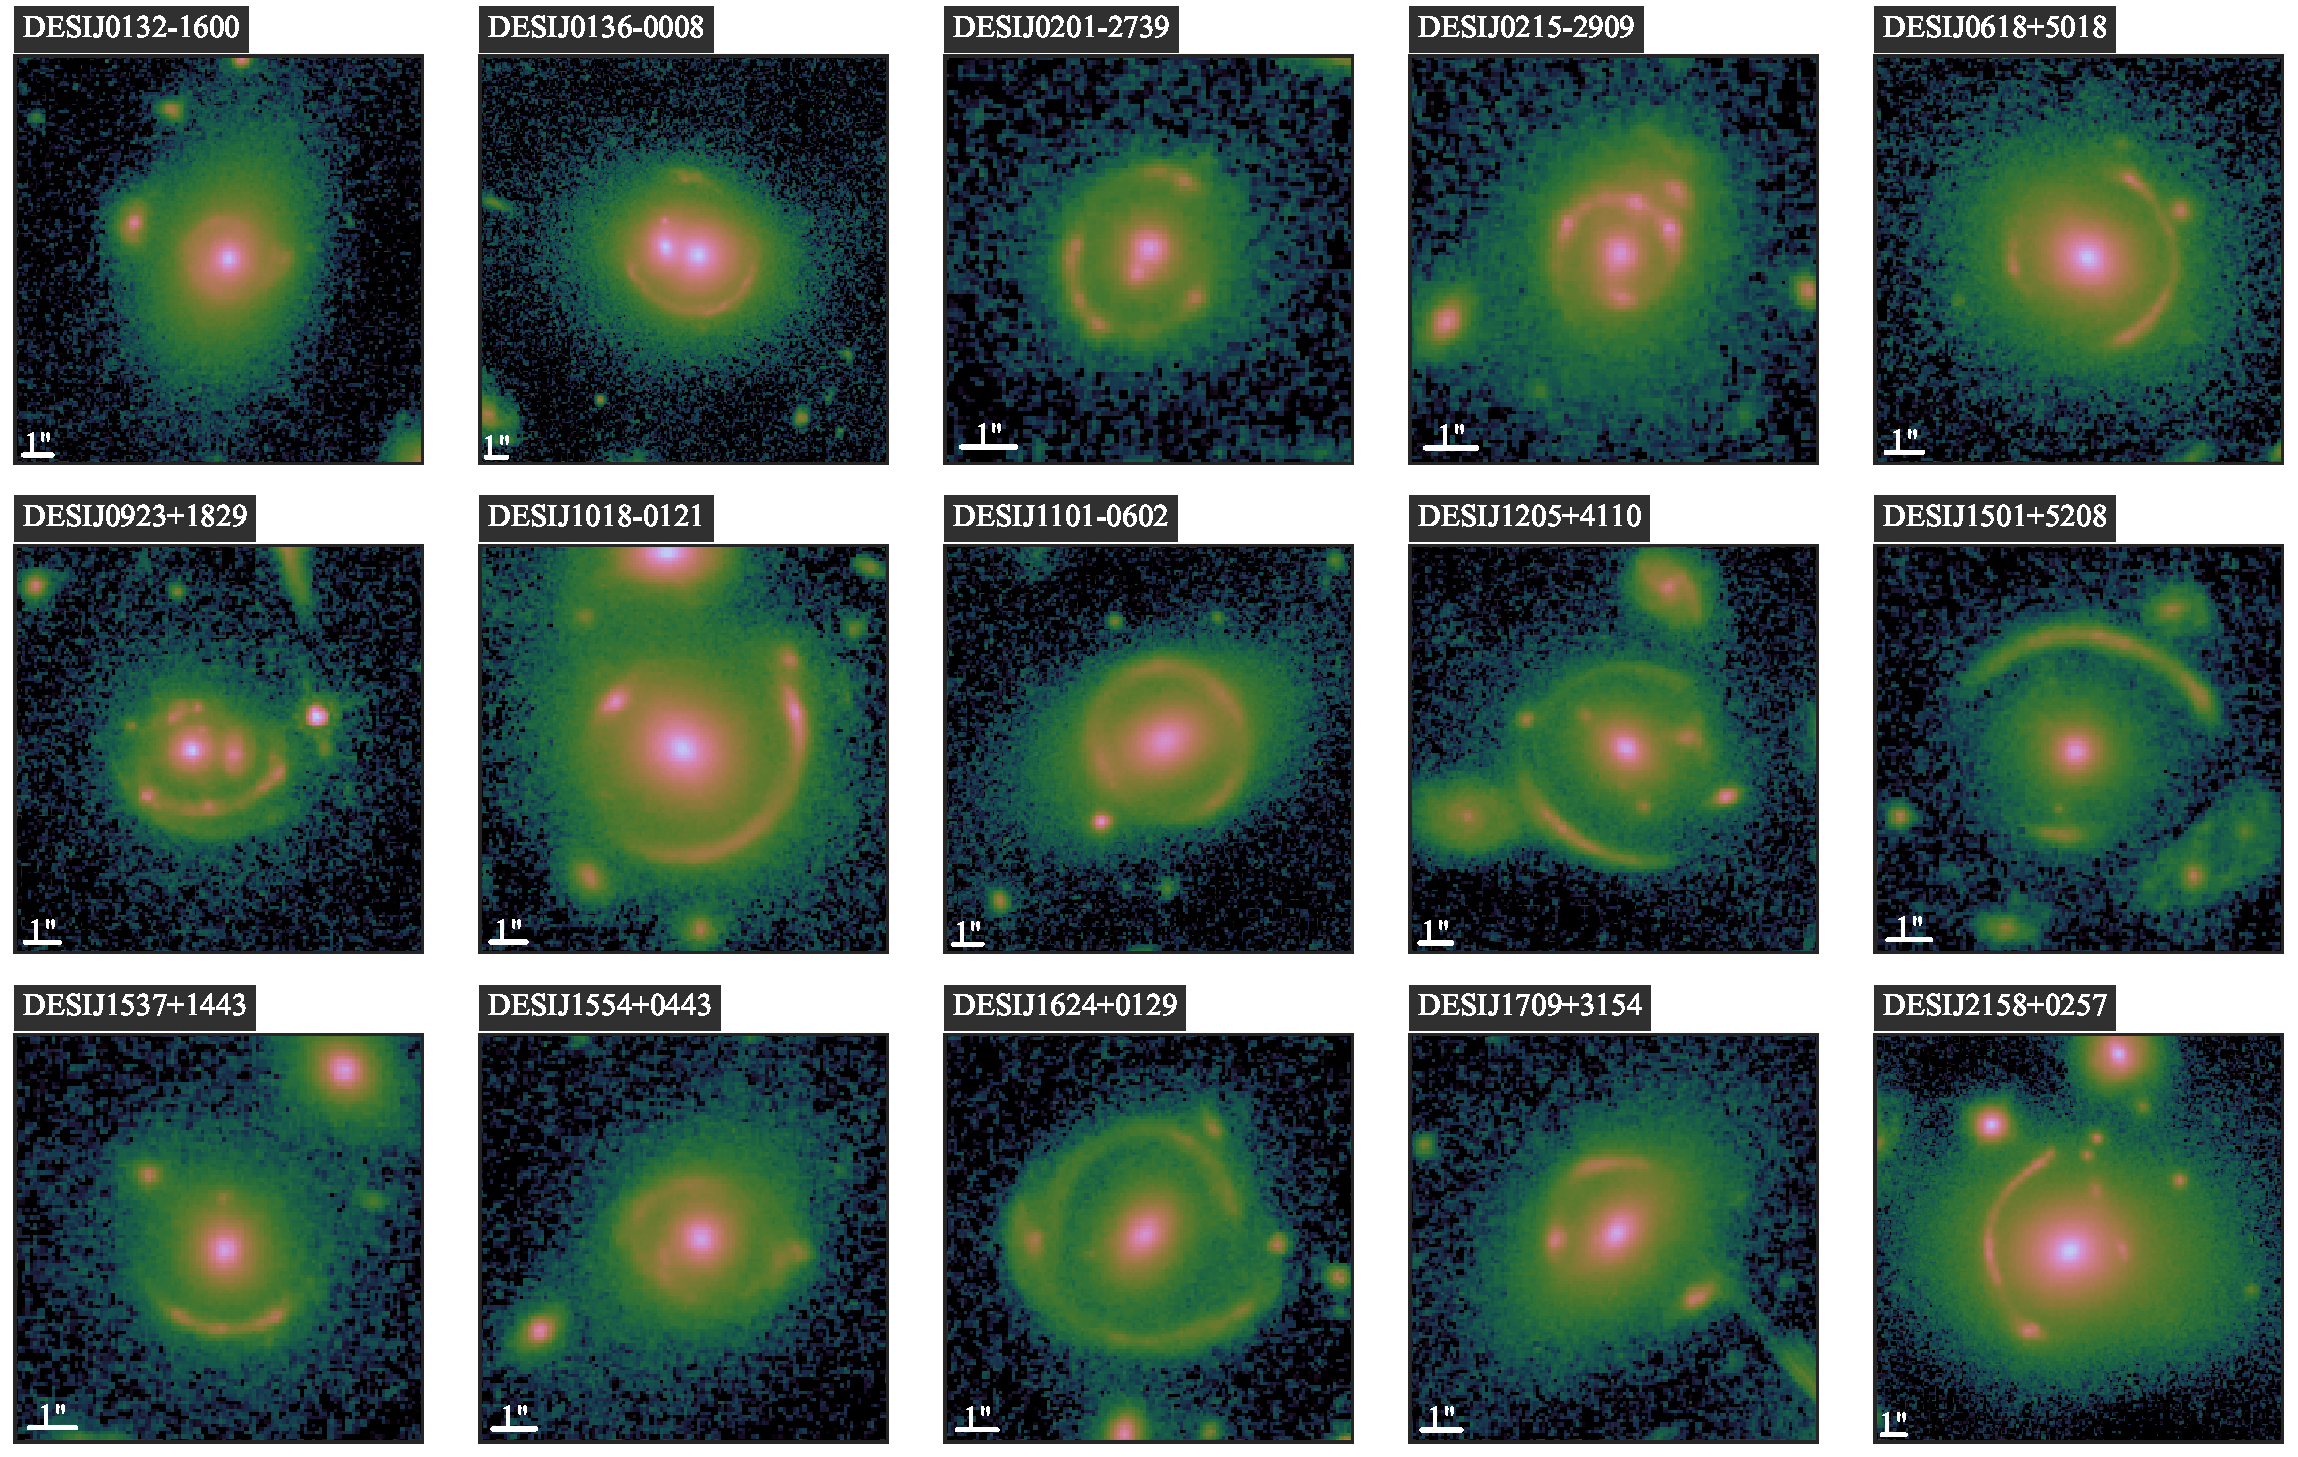
\includegraphics[width=\textwidth]{figures/lens_montage.pdf}
	\caption{\label{fig:montage}
	Montage of all the lens systems.
	}
\end{figure*}

\subsubsection{DESIJ0132$-$1600}
% Anik's Model

The central deflector in this system produces a lensing effect resembling a ring shape. Except for one conspicuous large object to the left of the lensing system, all other noticeable objects have been masked out. When modeling the source light of the system, we solely utilised the SHAPELETS profile, while the lens mass and light were modeled using EPL and S\'ersic profiles, respectively.

\subsubsection{DESIJ0136$-$0008}
% Akbar's Model

This system has two lensing galaxies of comparable sizes within the Einstein radius. Another smaller object also exists within the Einstein radius, which is potentially a third-member galaxy within this group. We model the larger galaxy on the west as the main deflector. We also explicitly modeled the mass profile of the large companion with a SIE model. However, we assumed the lensing effect of the potential third group member is negligible, given its relatively smaller size and it not being in close proximity to the arcs, by masking over its light. We also noticed some prominent residual in between the two largest galaxies that the smooth S\'ersic profiles were not adequate to describe. This non-smooth structure may potentially arise if these two galaxies are interacting or merging. We masked this non-smooth structure in the light distribution (Figure \ref{fig:lens_models_0}).

\subsubsection{DESIJ0201$-$2739} \label{model:2739}
% Rafee's Model

In this system, an elliptical lensing effect is evident, showing a major central component and a minor one. We attribute the primary lensing arc to the significant central galaxy while considering the contribution of the minor central galaxy using an SIE mass profile. To encompass both companions, we adopted a double S\'ersic  profile to model the central galaxy and a single S\'ersic  profile to model the other one. To focus solely on the lensing contribution, we masked out a small source on the northwest side of the arc. Ultimately, the model generated a comprehensive elliptical ring for the system.

\subsubsection{DESIJ0215$-$2909}
% Milli's Model

At first glance, this lensing system appears to exhibit a spiral structure. Although it has a resemblance to a quad-system, its notable lensing effect qualifies it as a strong lensing candidate. Prior to modeling, we masked out a blob near the southeast corner and a light structure near the northwest. This modeling approach required the introduction of a double SHAPELETS profile to accurately represent the source contribution.

\subsubsection{DESIJ0618$-$5018}
% Nishuti's Model
% to be written
Compared to other systems in our sample, this model exhibits striking similarities, featuring a prominent arc to the west of the central deflector, accompanied by a discernible counter image. Following our initial estimation, we identified the need to address a nearby blob serving as our satellite galaxy in the north-western position, necessitating the incorporation of an SIE model and corresponding S\'ersic profile. Additionally, we encountered an undesired light source in the upper corner of our major arc, requiring masking. Two similar blobs were also masked to refine the model further.


\subsubsection{DESIJ0923$+$1829}
% Mamunur rashid's Model

In this model, we observe two central deflectors contributing to the formation of two distinct lensing features. To streamline the model, we masked the crescent-shaped lens arc created by the minor deflector. To ensure better accuracy, we recognised the need to mask the surrounding region of the satellite. Consequently, we modeled the mass of the satellite galaxy using an SIE profile and introduced a third S\'ersic profile to assist in its light modeling. Additionally, to enhance precision, we masked clearly discernible stars accompanied by diffraction spikes.

\subsubsection{DESIJ1018$-$0121}
% Jobair's Model

We assumed the arc spanning from around the northwest position to around the southeast position as the main component of the gravitational lensing arc with a smaller blob at around the northeast as its counter image. Masking was done by covering non-lensing elements of the image. The system is surrounded by some stars and galaxies which are masked out.


\subsubsection{DESIJ1101$-$0602}
% Nishi's Model (under Rafee)

This particular system exhibits the most circular and well-defined Einstein ring among all the models we've analyzed. Adjacent to the Einstein ring, a circular blob is evident near the southeast, clearly unrelated to the system itself. To ensure accurate modeling, we masked this blob along with two additional objects due south. Throughout the modeling process, it became apparent that the central deflector was generating some extraneous lights, which we considered unnecessary and subsequently masked. It's worth noting that only the baseline models were employed in this analysis.

\subsubsection{DESIJ1205$+$4110}
\newcommand{\suggestion}[1]{\textcolor{blue}{#1}}
% Robin's Model

Within this system, a prominent central galaxy is accompanied by multiple smaller galaxies positioned within its Einstein radius. We treated the nearby smaller galaxies as having negligible lensing effects, masking over their lights due to their size disparity and distance from the observed arcs. Employing an EPL and SHEAR model, we designated the central galaxy as the primary deflector. However, to accurately reproduce the triangular-shaped arc due northwest, this choice of mass models proved insufficient. Acknowledging the presence of nearby large elliptical galaxies outside the Einstein radius, we introduced a FLEXION model to incorporate their lensing effects. This adjustment successfully accounted for all arcs, including the distorted one.


\subsubsection{DESIJ1501$+$5208}
% Nahid's model

This system exhibits a crescent-shaped major lensing effect, complemented by its counter-image, indicating its candidacy as a strong lensing system. We observed a very faint object near the counter image, but we excluded it from the lensing system during the modeling process. Additionally, several objects located outside the Einstein radius were also masked. Our modeling approach involved only the baseline models. Despite our efforts, we encountered difficulty in identifying suitable parameters to model certain residual blue features within the Einstein radius. However, these features did not significantly affect the lensing parameters themselves.

\subsubsection{DESIJ1537$+$1443}
% Tanver's model

This system prominently displays a strong lensing arc towards the south of the main deflector. The primary gravitational lensing structure extends approximately from the southwest position to around the southeast, accompanied by a smaller blob positioned due north, serving as its corresponding counter image. However, the proximity of the lensing system to another galaxy blob in the northwest necessitated its exclusion through masking during the modeling process. Additionally, a smaller mask was applied close to the northeast. We employed only the baseline profiles to construct the lenses during the modeling phase.

\subsubsection{DESIJ1554$+$0443}
% Zareef's Model

In this lensing system, the system itself is relatively small, with a diameter of approximately 4 arcseconds. During modeling, we masked only a blob located near the southeast. Standard mass profiles and light profiles like EPL and S\'ersic  were utilized in this analysis. Two prominent arc features were observed, and following the modeling process, these features formed a complete elliptical ring.

\subsubsection{DESIJ1624$+$0129}
% Imtiaz's model

This system exhibits prominent lensing effects with a well-defined major lensing component and its corresponding counter-image, clearly distinguishable. Our model detected a satellite companion westward position, which we addressed using the SIE profile. Additional elements positioned outside the Einstein radius, particularly towards the south and near the southwest direction, were excluded. However, upon completing the modeling process, we identified the need for further masking above the arcs themselves. Although this additional masking did not significantly alter the intended parameters for the lens, it did contribute to the overall system's light.


\subsubsection{DESIJ1709$+$3154}
% tanzilla's model

In this lensing system, three prominent arc features have been observed and modeled using our baseline models. Additionally, there are some light features in the southeast, identified as diffraction spikes from a nearby large line of sight star. To eliminate these effects, we utilized masking techniques. Furthermore, a very faint object located to the right of the lensing system has also been masked.

\subsubsection{DESIJ2158$+$0257}
% Fahim's Model

In this system, various objects reside within a densely populated area encompassing the Einstein radius. A significant arc is discernible, formed by the central deflector on the left side with its corresponding counter image on the right. To ensure accurate modeling, we strategically masked two regions within the Einstein radius and several larger nearby objects/stars, excluding contributions from line-of-sight objects and stars with diffraction spikes. Upon closer examination during modeling, we identified additional light sources near the south-west. These were present in the observed system but did not appear to be associated with any stars or our lensing system. Consequently, we decided to mask out this particular region. The central lens mass was modeled using the EPL method, while a double S\'ersic profile was employed to model the lens light.

\section{Result} \label{sec:result}
In this section, we present the best-fit values of both the lens model and the photometric parameters. The lens model parameters are the Einstein radius ($\theta_{E}$), the logarithmic slope $\gamma$, the mass ellipticity and position angle ($q_{m}$ and $\phi_{m}$), the light ellipticity and position angle ($q_{L}$ and $\phi_{L}$), the 'external' shears ($\gamma_{shear}$ and $\phi_{shear}$) and the effective or half-light radius $R_{eff}$. 
The photometric parameters are $\Sigma_{10}$, $\Sigma_{10, \text{flux selected}}$, $\Sigma_{20}$, and $\Sigma_{20, \text{flux selected}}$.
During analyses, we use the lens model parameters as measures of internal structural properties and the photometric parameters as the measures of the environments surrounding the deflectors.

\subsection{Lens model parameters}
After acquiring the best-fit values of the lens model parameters, we present the parameters directly relevant to our analyses in Table \ref{table:lens_params}. The Einstein radii represent the size of the deflectors ($\theta_{E}$ parametrizes the lens mass profile). The $\gamma$ values embed information on the distributions of dark and hadronic matters. The light and mass ellipticies show a strong correlation. We check the offsets between the mass and light position angles for correlation with the source density measures. $R_{eff}$ indicates the angular size of the lenses. The `external shear' parameters $\gamma_{shear}$ and $\phi_{shear}$ are not used in the analyses as \cite{etherington23} points toward an inadequacy in their representation of the physical shear. Instead, we use the photometric source-density measures ($\Sigma$s) denoting the densities considering a certain number of nearest sources.
\begin{figure*}
	\centering
	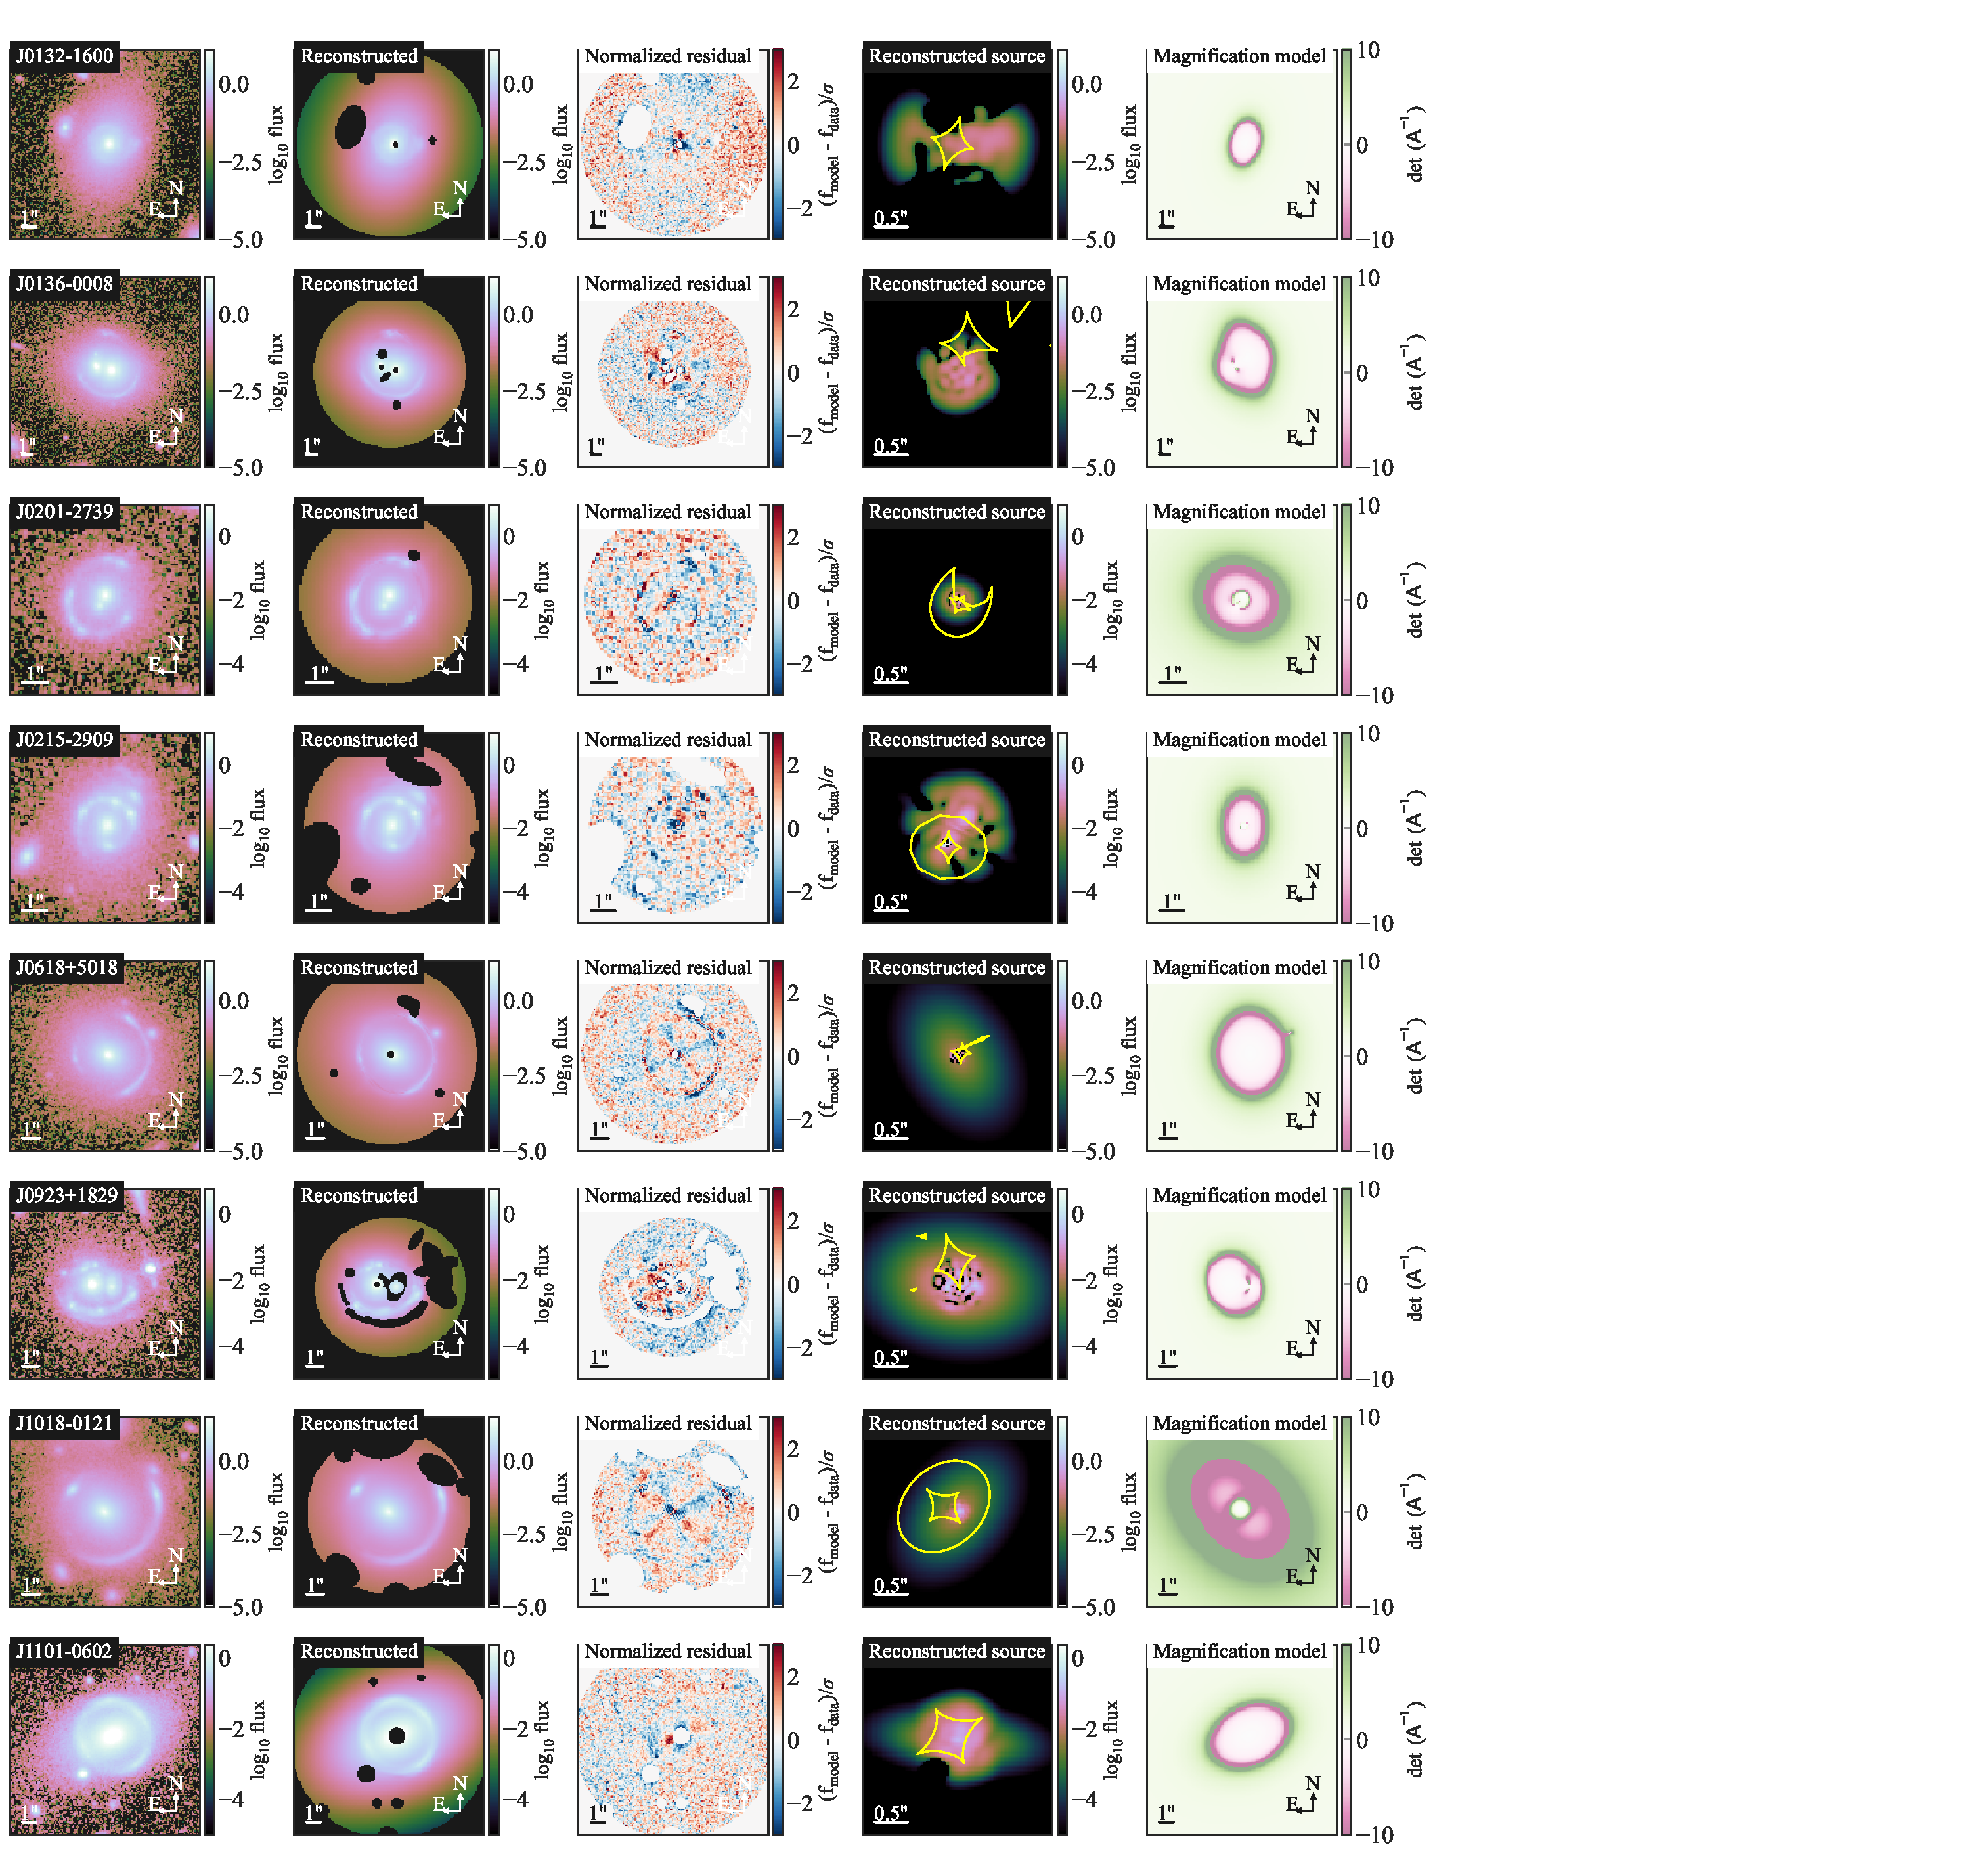
\includegraphics[width=1.5\textwidth]{paper/figures/lens_models_0.pdf}
	\caption{\label{fig:lens_models_0}
	Illustration of the lens models for the lens systems in our sample.
	}
\end{figure*}

\begin{figure*}\ContinuedFloat
	\centering
	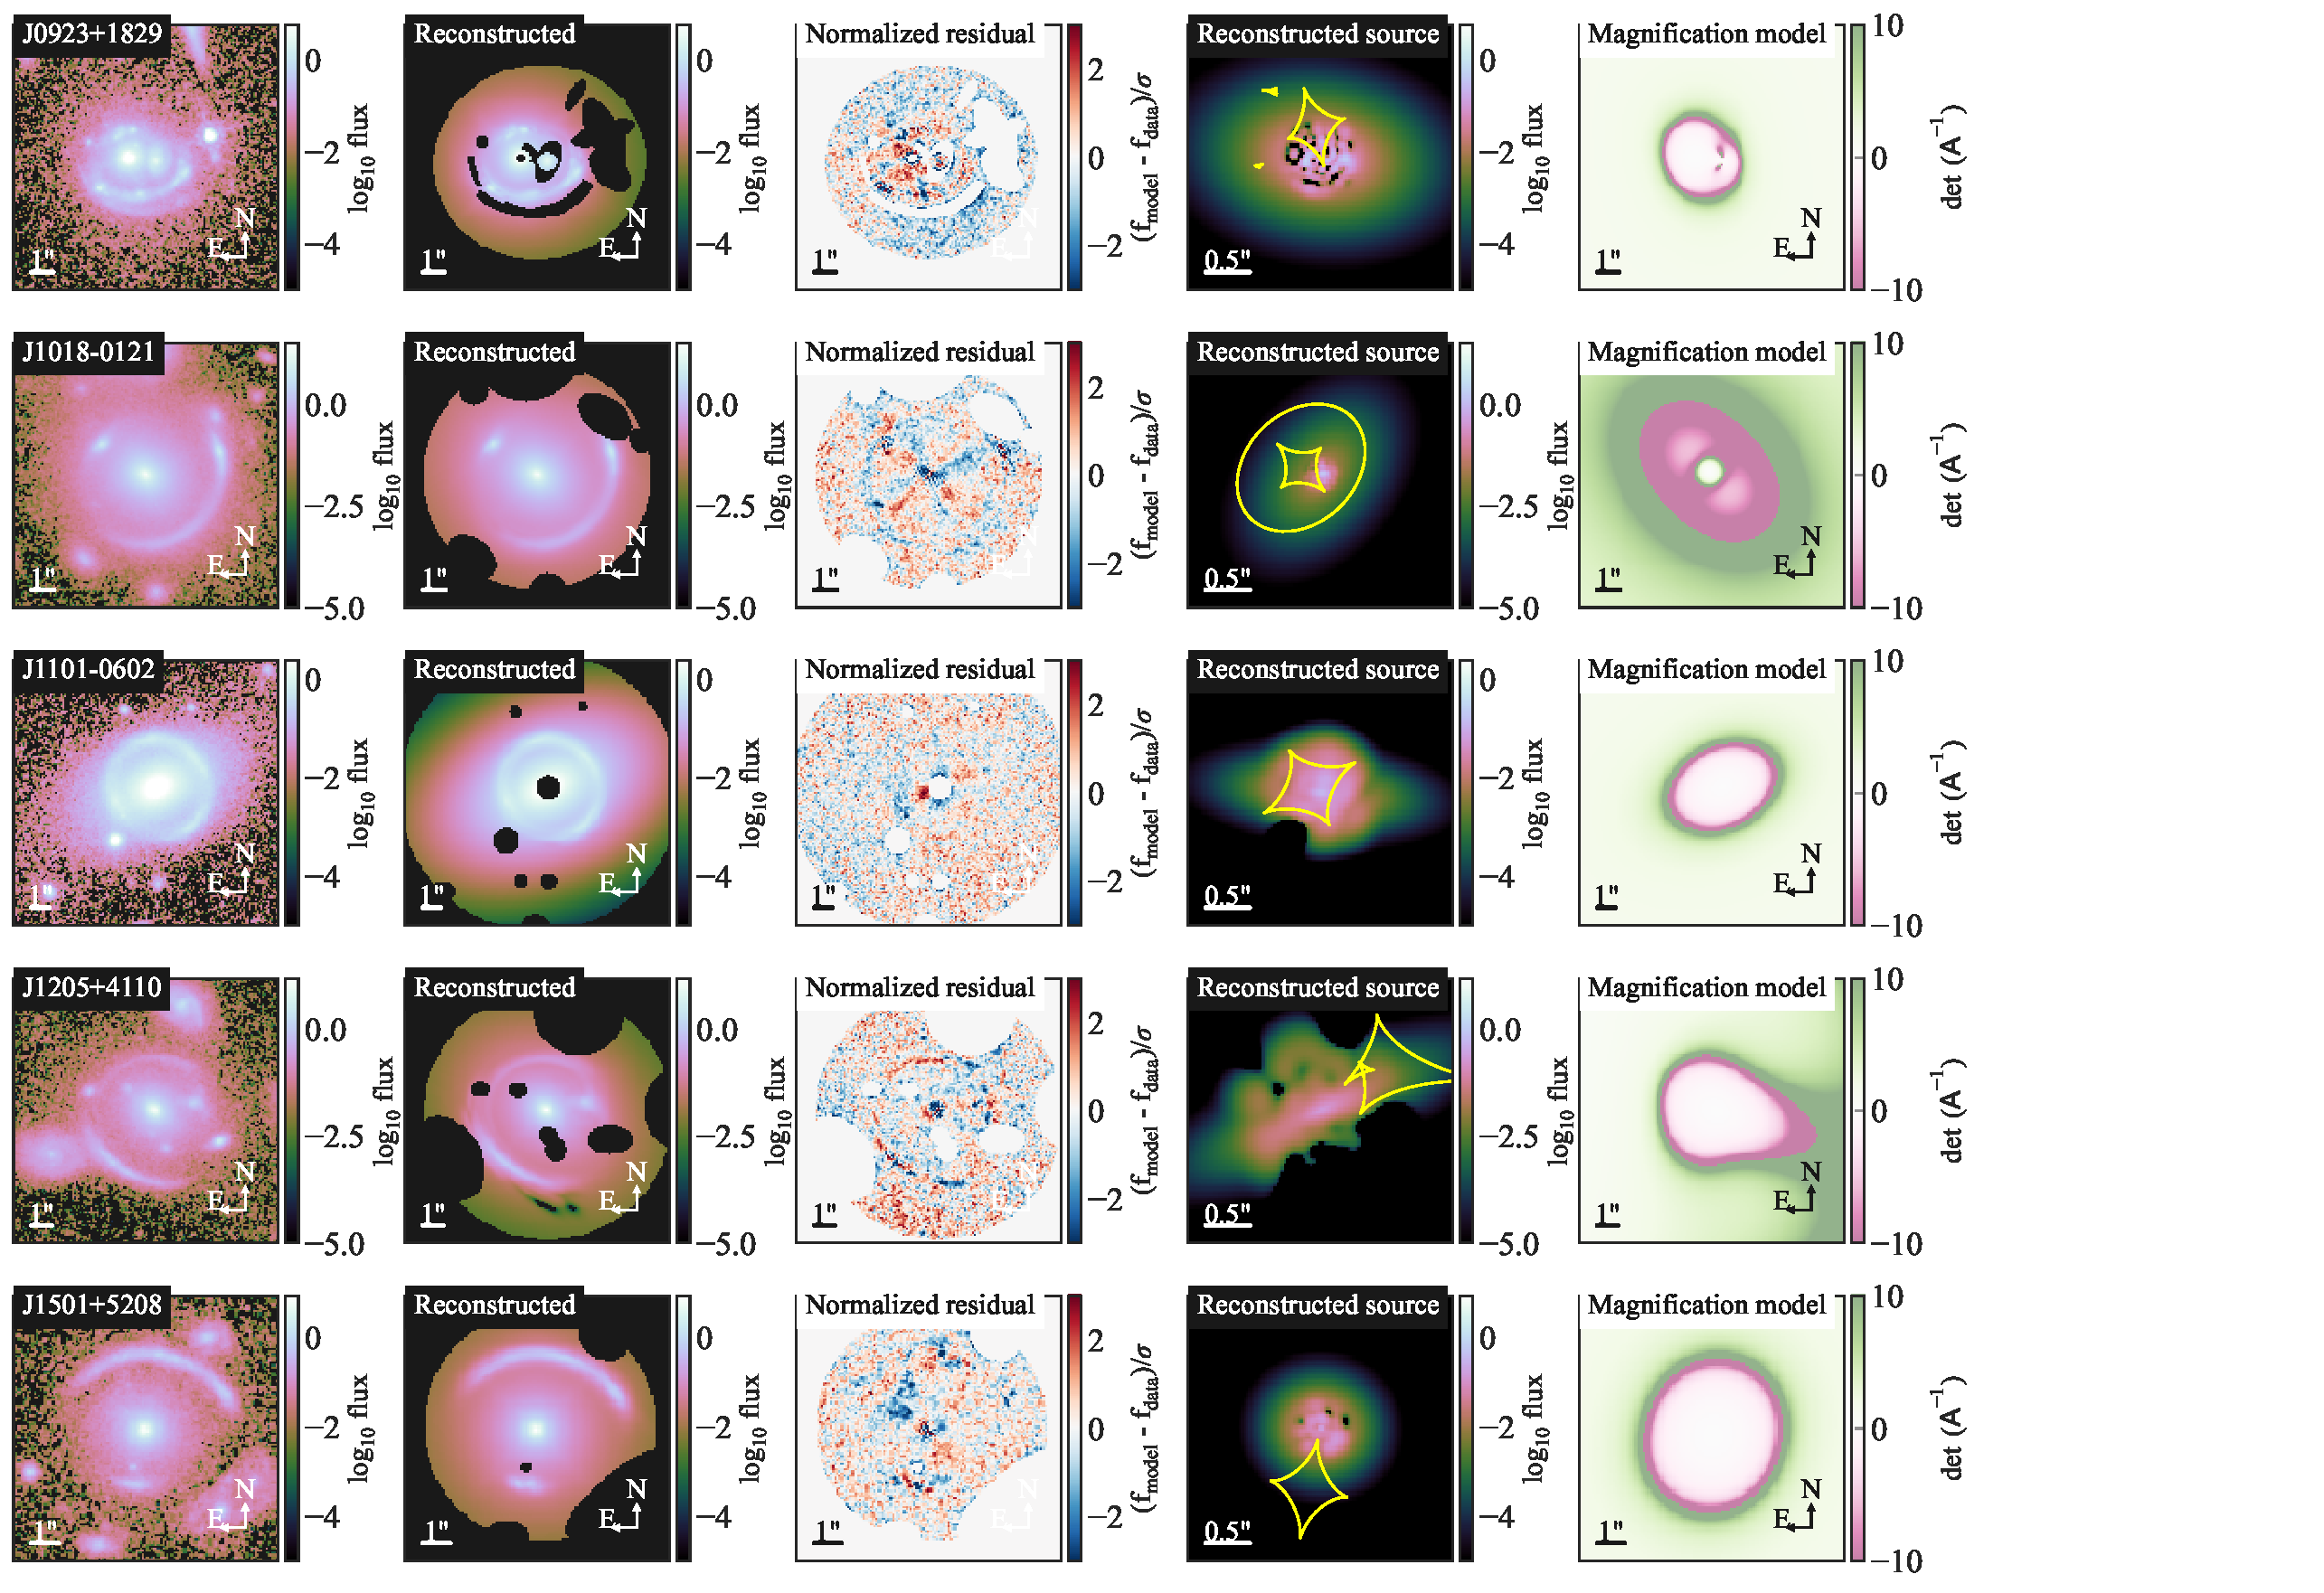
\includegraphics[width=1.40\textwidth]{paper/figures/lens_models_1.pdf}
	\caption{\label{fig:lens_models_1}
	Illustration of the lens models for the lens systems in our sample (continued).
	}
\end{figure*}

\renewcommand{\arraystretch}{1.3}
 \begin{table*}
 \caption{Lens model parameters: $\theta_{\rm E}$ is the Einstein radius, $\gamma$ is the logarithmic slope of the mass profile, $q_{\rm m}$ is the mass axis ratio, $\phi_{\rm m}$ is the major axis position angle for mass,  $\gamma_{\rm shear}$ is the residual shear magnitude and $\phi_{\rm shear}$ is the residual shear angle,
 $R_{\rm eff}$ is the effective radius of the light profile,  $q_{\rm L}$ is the light axis ratio, and $\phi_{\rm L}$ is the major axis position angle for light. The angles $\phi_{\rm m}$, $\phi_{\rm shear}$, and $\phi_{\rm L}$ are defined as \textcolor{red}{X of X}. The point estimates are the medians of the 1D marginalized posteriors and the 1$\sigma$ uncertainties are obtained from the 16th and 84th percentiles.
\label{table:lens_params}
}
\centering
\begin{tabular}{lccccccccc}
\hline
     System &  $\theta_{\rm E}$ &    $\gamma$ &    $q_\text{m}$ &     $\phi_\text{m}$ &  $\gamma_\text{shear}$  &  $\phi_\text{shear}$  &
     $R_{\rm eff} $ & 
     $q_\text{L}$ & 
     $\phi_\text{L}$
     \\
     & (\arcsec) & & &(\degr)   & & (\degr) & (\arcsec) & & (\degr) \\
\hline
% column values go into lens_model_param.tex file
J0136$-$0008 &         $2.711_{-0.009}^{+0.008}$ &         $2.01_{-0.02}^{+0.02}$ &         $0.538_{-0.004}^{+0.005}$ &         $70.0_{-0.3}^{+0.3}$ &         $0.134_{-0.003}^{+0.003}$ &         $62.1_{-0.5}^{+0.5}$ &         $0.98 \pm 0.02$ &         $0.900_{-0.001}^{+0.001}$ &         $10.5_{-0.3}^{+0.3}$ \\ 
J0215$-$2909 &         $1.055_{-0.001}^{+0.002}$ &         $1.80_{-0.02}^{+0.01}$ &         $0.717_{-0.005}^{+0.008}$ &         $-88.8_{-0.4}^{+0.5}$ &         $0.011_{-0.003}^{+0.002}$ &         $-81.8_{-4.4}^{+5.6}$ &         $0.92 \pm 0.02$ &         $0.794_{-0.004}^{+0.004}$ &         $-78.9_{-0.7}^{+0.6}$ \\ 
J0618$+$5018 &             $2.265_{-0.001}^{+0.001}$ &             $2.00$ &             $0.726_{-0.002}^{+0.003}$ &             $83.3_{-0.3}^{+0.3}$ &             $0.074_{-0.001}^{+0.001}$ &             $79.1_{-0.4}^{+0.5}$ &             $0.82 \pm 0.02$ &             $0.792_{-0.002}^{+0.002}$ &             $31.4_{-0.3}^{+0.4}$ \\ 
J1018$-$0121 &         $2.915_{-0.002}^{+0.002}$ &         $1.49_{-0.01}^{+0.01}$ &         $0.727_{-0.005}^{+0.005}$ &         $45.5_{-0.3}^{+0.3}$ &         $0.079_{-0.002}^{+0.002}$ &         $45.7_{-0.5}^{+0.6}$ &         $1.23 \pm 0.02$ &         $0.815_{-0.002}^{+0.001}$ &         $37.3_{-0.2}^{+0.2}$ \\ 
J1205$+$4110 &         $2.815_{-0.007}^{+0.007}$ &         $2.05_{-0.02}^{+0.03}$ &         $0.631_{-0.009}^{+0.008}$ &         $27.3_{-0.7}^{+0.7}$ &         $0.096_{-0.005}^{+0.004}$ &         $39.7_{-1.0}^{+0.8}$ &         $0.89 \pm 0.02$ &         $0.793_{-0.002}^{+0.003}$ &         $39.0_{-0.4}^{+0.5}$ \\ 
J1501$+$5208 &         $2.603_{-0.004}^{+0.004}$ &         $2.08_{-0.03}^{+0.03}$ &         $0.830_{-0.022}^{+0.026}$ &         $-4.0_{-2.7}^{+2.1}$ &         $0.147_{-0.009}^{+0.008}$ &         $5.1_{-0.6}^{+0.6}$ &         $0.72 \pm 0.01$ &         $0.953_{-0.005}^{+0.005}$ &         $26.9_{-3.3}^{+3.0}$ \\ 
J1537$+$1443 &         $1.552_{-0.016}^{+0.006}$ &         $2.06_{-0.08}^{+0.07}$ &         $0.656_{-0.017}^{+0.025}$ &         $-86.0_{-3.7}^{+175.7}$ &         $-0.748_{-0.308}^{+0.283}$ &         $1.4_{-0.3}^{+0.7}$ &         $0.71 \pm 0.01$ &         $0.880_{-0.004}^{+0.004}$ &         $76.6_{-0.9}^{+0.9}$ \\ 
J1554$+$0443 &         $1.502_{-0.005}^{+0.004}$ &         $1.85_{-0.02}^{+0.02}$ &         $0.800_{-0.011}^{+0.013}$ &         $-55.3_{-2.3}^{+2.2}$ &         $0.106_{-0.006}^{+0.005}$ &         $6.8_{-1.3}^{+1.5}$ &         $0.78 \pm 0.02$ &         $0.919_{-0.002}^{+0.002}$ &         $-49.4_{-0.7}^{+0.8}$ \\ 
J1624$+$0129 &         $2.683_{-0.004}^{+0.004}$ &         $1.71_{-0.05}^{+0.05}$ &         $0.828_{-0.007}^{+0.008}$ &         $-50.2_{-0.8}^{+0.8}$ &         $0.041_{-0.004}^{+0.003}$ &         $-42.8_{-1.3}^{+1.3}$ &         $0.79 \pm 0.02$ &         $0.698_{-0.003}^{+0.002}$ &         $-56.4_{-0.3}^{+0.4}$ \\ 
J1709$+$3154 &         $2.029_{-0.004}^{+0.004}$ &         $1.74_{-0.02}^{+0.02}$ &         $0.678_{-0.012}^{+0.011}$ &         $-36.3_{-0.5}^{+0.6}$ &         $0.040_{-0.004}^{+0.004}$ &         $-18.2_{-2.5}^{+2.8}$ &         $0.89 \pm 0.02$ &         $0.619_{-0.002}^{+0.002}$ &         $-46.7_{-0.2}^{+0.2}$ \\ 
J2158$+$0257 &         $3.319_{-0.004}^{+0.004}$ &         $1.94_{-0.03}^{+0.03}$ &         $0.763_{-0.004}^{+0.004}$ &         $-18.3_{-0.6}^{+0.7}$ &         $0.112_{-0.005}^{+0.005}$ &         $-75.1_{-0.8}^{+1.0}$ &         $1.22 \pm 0.02$ &         $0.905_{-0.000}^{+0.001}$ &         $-8.1_{-0.1}^{+0.2}$ \\ 
\hline
 
\end{tabular}
\end{table*}

\renewcommand{\arraystretch}{1.3}
 \begin{table*}
 \caption{Photometric parameters: $\Sigma_{10}$ is the source density considering the nearest 10 neighbors, $\Sigma_{10,\text{flux selected}}$ is the source density considering the nearest 10 neighbors having fluxes greater than 1\% of the central deflector's, $\Sigma_{20}$ is the source density considering the nearest 20 neighbors, $\Sigma_{20,\text{flux selected}}$ is the source density considering the nearest 20 neighbors having fluxes greater than 1\% of the central deflector's,
\label{table:photometric_params}
}
\centering
\begin{tabular}{lccccccccc}
\hline
     System & Redshift(z) &  $\Sigma_{10}$ &    $\Sigma_{10,\text{flux selected}}$ &    $\Sigma_{20}$ &     $\Sigma_{20,\text{flux selected}}$ & centroid offset  & position-angle offset \\
     & & (\arcsec^{-2}) & (\arcsec^{-2}) & (\arcsec^{-2}) & (\arcsec^{-2}) & (\arcsec)  & (\degr)  \\
\hline
% column values go into photometric_params.tex file
J0132$-$1600 &             $0.36 \pm 0.04$ &             $647 \pm 99$ &             $56 \pm 9$ &             $853 \pm 132$ &             $82 \pm 13$ &            $0.73 \pm 0.07$ &             $4.1 \pm 2.5$ & \\ 
J0136$-$0008 &             $0.34 \pm 0.04$ &             $389 \pm 56$ &             $61 \pm 9$ &             $533 \pm 77$ &             $82 \pm 12$ &            $6.09 \pm 0.42$ &             $59.5 \pm 0.4$ & \\ 
J0201$-$2739 &             $0.75 \pm 0.07$ &             $1130 \pm 77$ &             $876 \pm 59$ &             $1245 \pm 85$ &             $723 \pm 49$ &            $0.39 \pm 0.06$ &             $44.8 \pm 12.6$ & \\ 
J0215$-$2909 &             $0.94 \pm 0.12$ &             $622 \pm 48$ &             $293 \pm 23$ &             $706 \pm 55$ &             $316 \pm 25$ &            $0.45 \pm 0.04$ &             $9.9 \pm 0.8$ & \\ 
J0618$+$5018 &             $0.52 \pm 0.08$ &             $1431 \pm 257$ &             $119 \pm 21$ &             $718 \pm 126$ &             $137 \pm 24$ &            $1.76 \pm 0.14$ &             $52.0 \pm 0.5$ & \\ 
J0923$+$1829 &             $0.68 \pm 0.05$ &             $455 \pm 30$ &             $226 \pm 15$ &             $400 \pm 26$ &             $242 \pm 16$ &            $0.27 \pm 0.04$ &             $66.1 \pm 19.6$ & \\ 
J1018$-$0121 &             $0.40 \pm 0.03$ &             $1011 \pm 92$ &             $322 \pm 29$ &             $997 \pm 90$ &             $127 \pm 12$ &            $0.97 \pm 0.04$ &             $8.2 \pm 0.4$ & \\ 
J1101$-$0602 &             $0.33 \pm 0.04$ &             $1568 \pm 284$ &             $168 \pm 31$ &             $1482 \pm 276$ &             $249 \pm 46$ &            $0.16 \pm 0.02$ &             $1.1 \pm 0.6$ & \\ 
J1205$+$4110 &             $0.62 \pm 0.02$ &             $514 \pm 16$ &             $234 \pm 8$ &             $514 \pm 16$ &             $223 \pm 7$ &            $1.50 \pm 0.10$ &             $11.7 \pm 0.8$ & \\ 
J1501$+$5208 &             $0.75 \pm 0.07$ &             $765 \pm 58$ &             $547 \pm 43$ &             $745 \pm 57$ &             $683 \pm 52$ &            $1.74 \pm 0.14$ &             $30.9 \pm 4.0$ & \\ 
J1537$+$1443 &             $0.65 \pm 0.04$ &             $425 \pm 24$ &             $312 \pm 18$ &             $556 \pm 32$ &             $454 \pm 26$ &            $0.58 \pm 0.18$ &             $13.4 \pm 1.4$ & \\ 
J1554$+$0443 &             $0.59 \pm 0.06$ &             $653 \pm 64$ &             $195 \pm 19$ &             $843 \pm 83$ &             $270 \pm 26$ &            $0.15 \pm 0.03$ &             $5.9 \pm 2.4$ & \\ 
J1624$+$0129 &             $0.79 \pm 0.05$ &             $788 \pm 34$ &             $534 \pm 23$ &             $819 \pm 35$ &             $363 \pm 16$ &            $1.13 \pm 0.04$ &             $6.2 \pm 0.9$ & \\ 
J1709$+$3154 &             $0.72 \pm 0.08$ &             $252 \pm 25$ &             $148 \pm 14$ &             $349 \pm 34$ &             $168 \pm 16$ &            $0.22 \pm 0.04$ &             $10.4 \pm 0.6$ & \\ 
J2158$+$0257 &             $0.28 \pm 0.02$ &             $1393 \pm 140$ &             $299 \pm 30$ &             $1489 \pm 149$ &             $88 \pm 9$ &            $0.66 \pm 0.04$ &             $10.2 \pm 0.6$ & \\ 
\hline
 
\end{tabular}
\end{table*}

\begin{figure}
    \resizebox{\hsize}{!}    {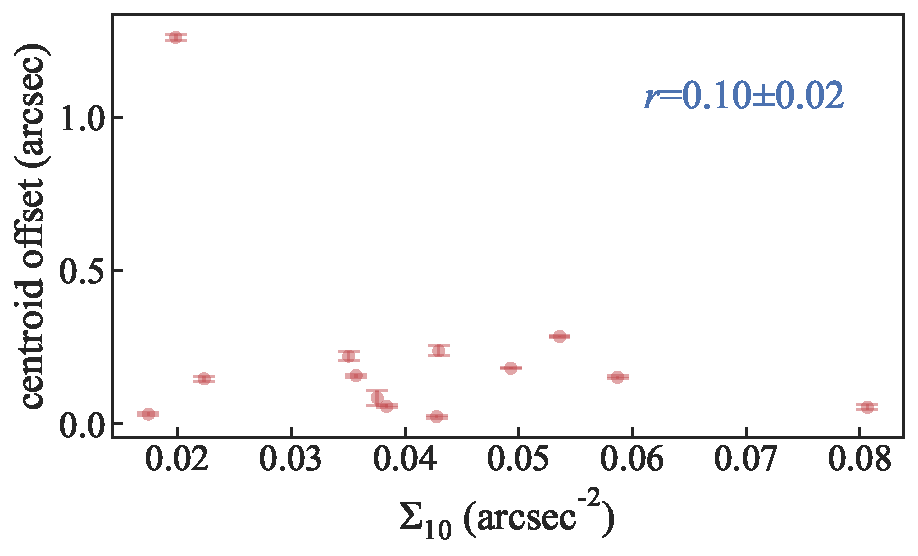
\includegraphics{paper/figures/centroid_offset_vs_Sigma_10.pdf}}    \caption{\label{fig:cent_off_Sigma_all}Centroid offset vs. $\Sigma_{10}$.}
\end{figure}

\begin{figure}
    \resizebox{\hsize}{!}    {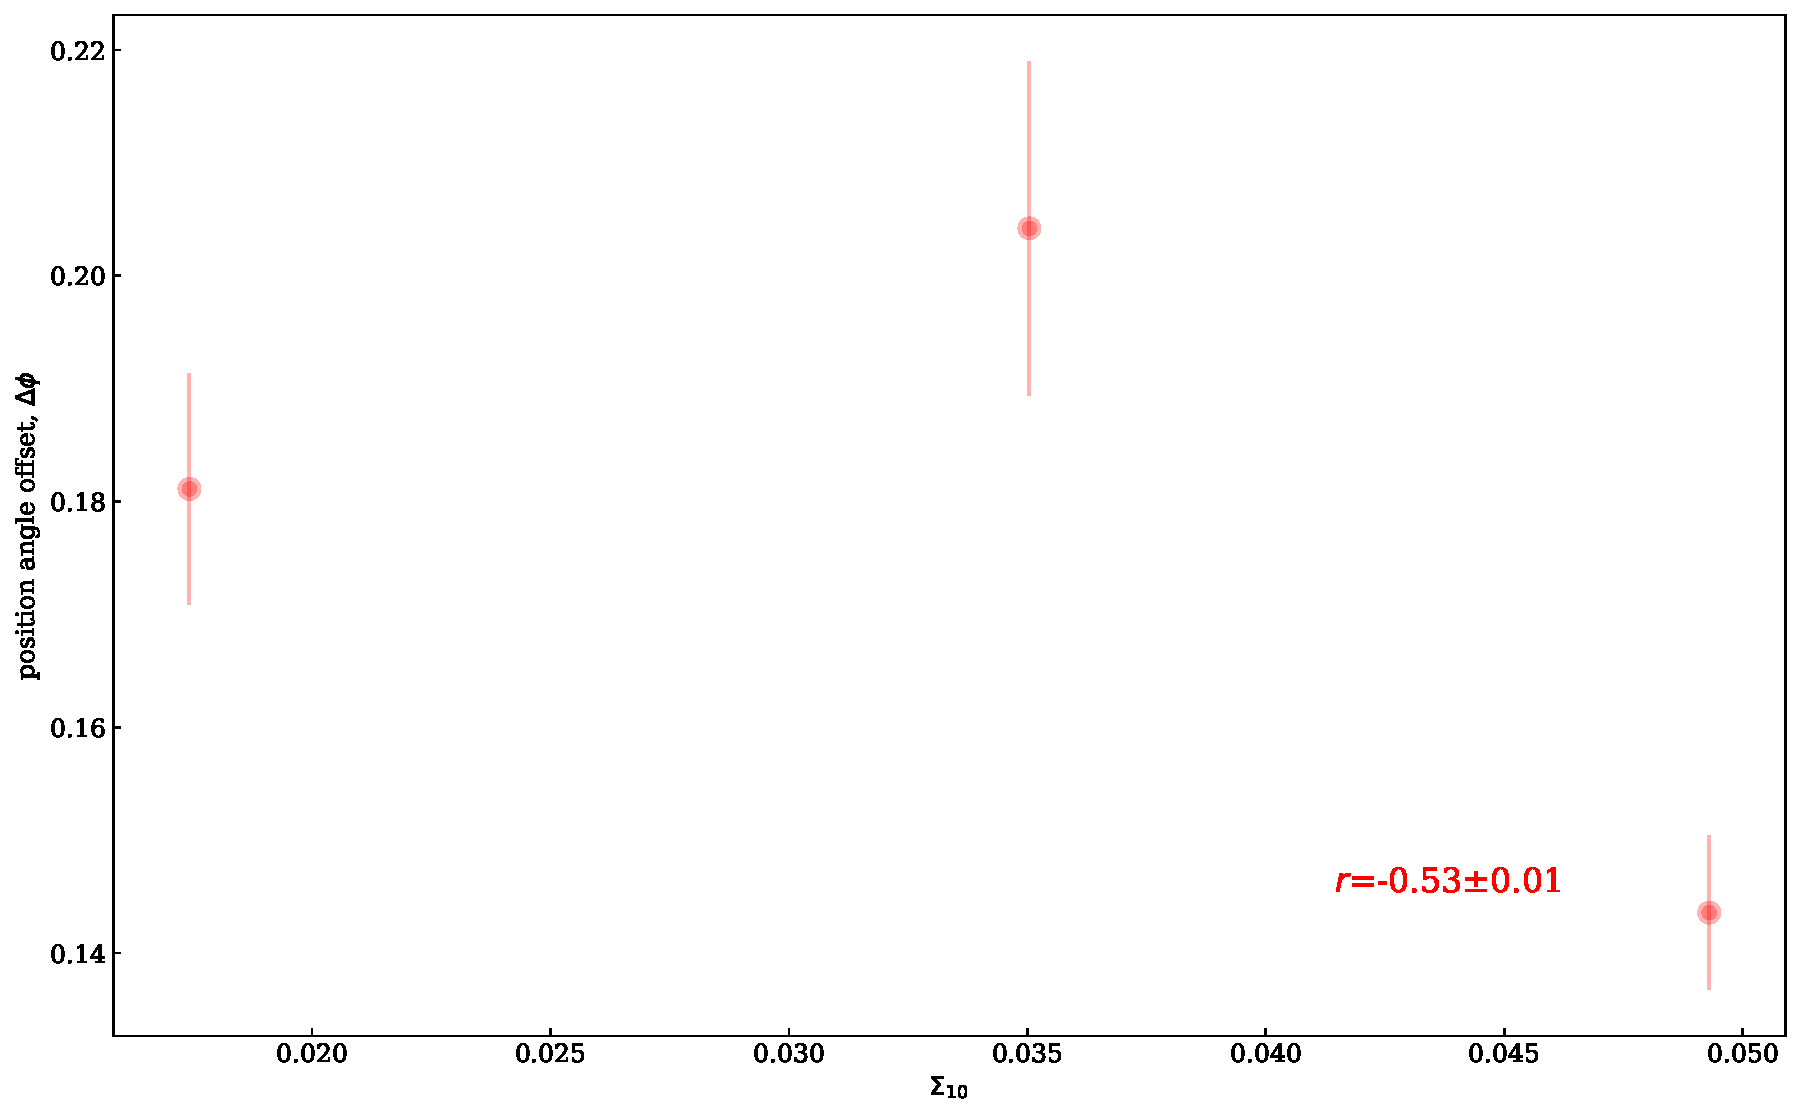
\includegraphics{paper/figures/position_angle_offset_vs_Sigma_10.pdf}}
    \caption{\label{fig:pos_off_Sigma_all}Position-angle offset vs. $\Sigma_{10}$.}
\end{figure}

\begin{figure*}
    \centering
    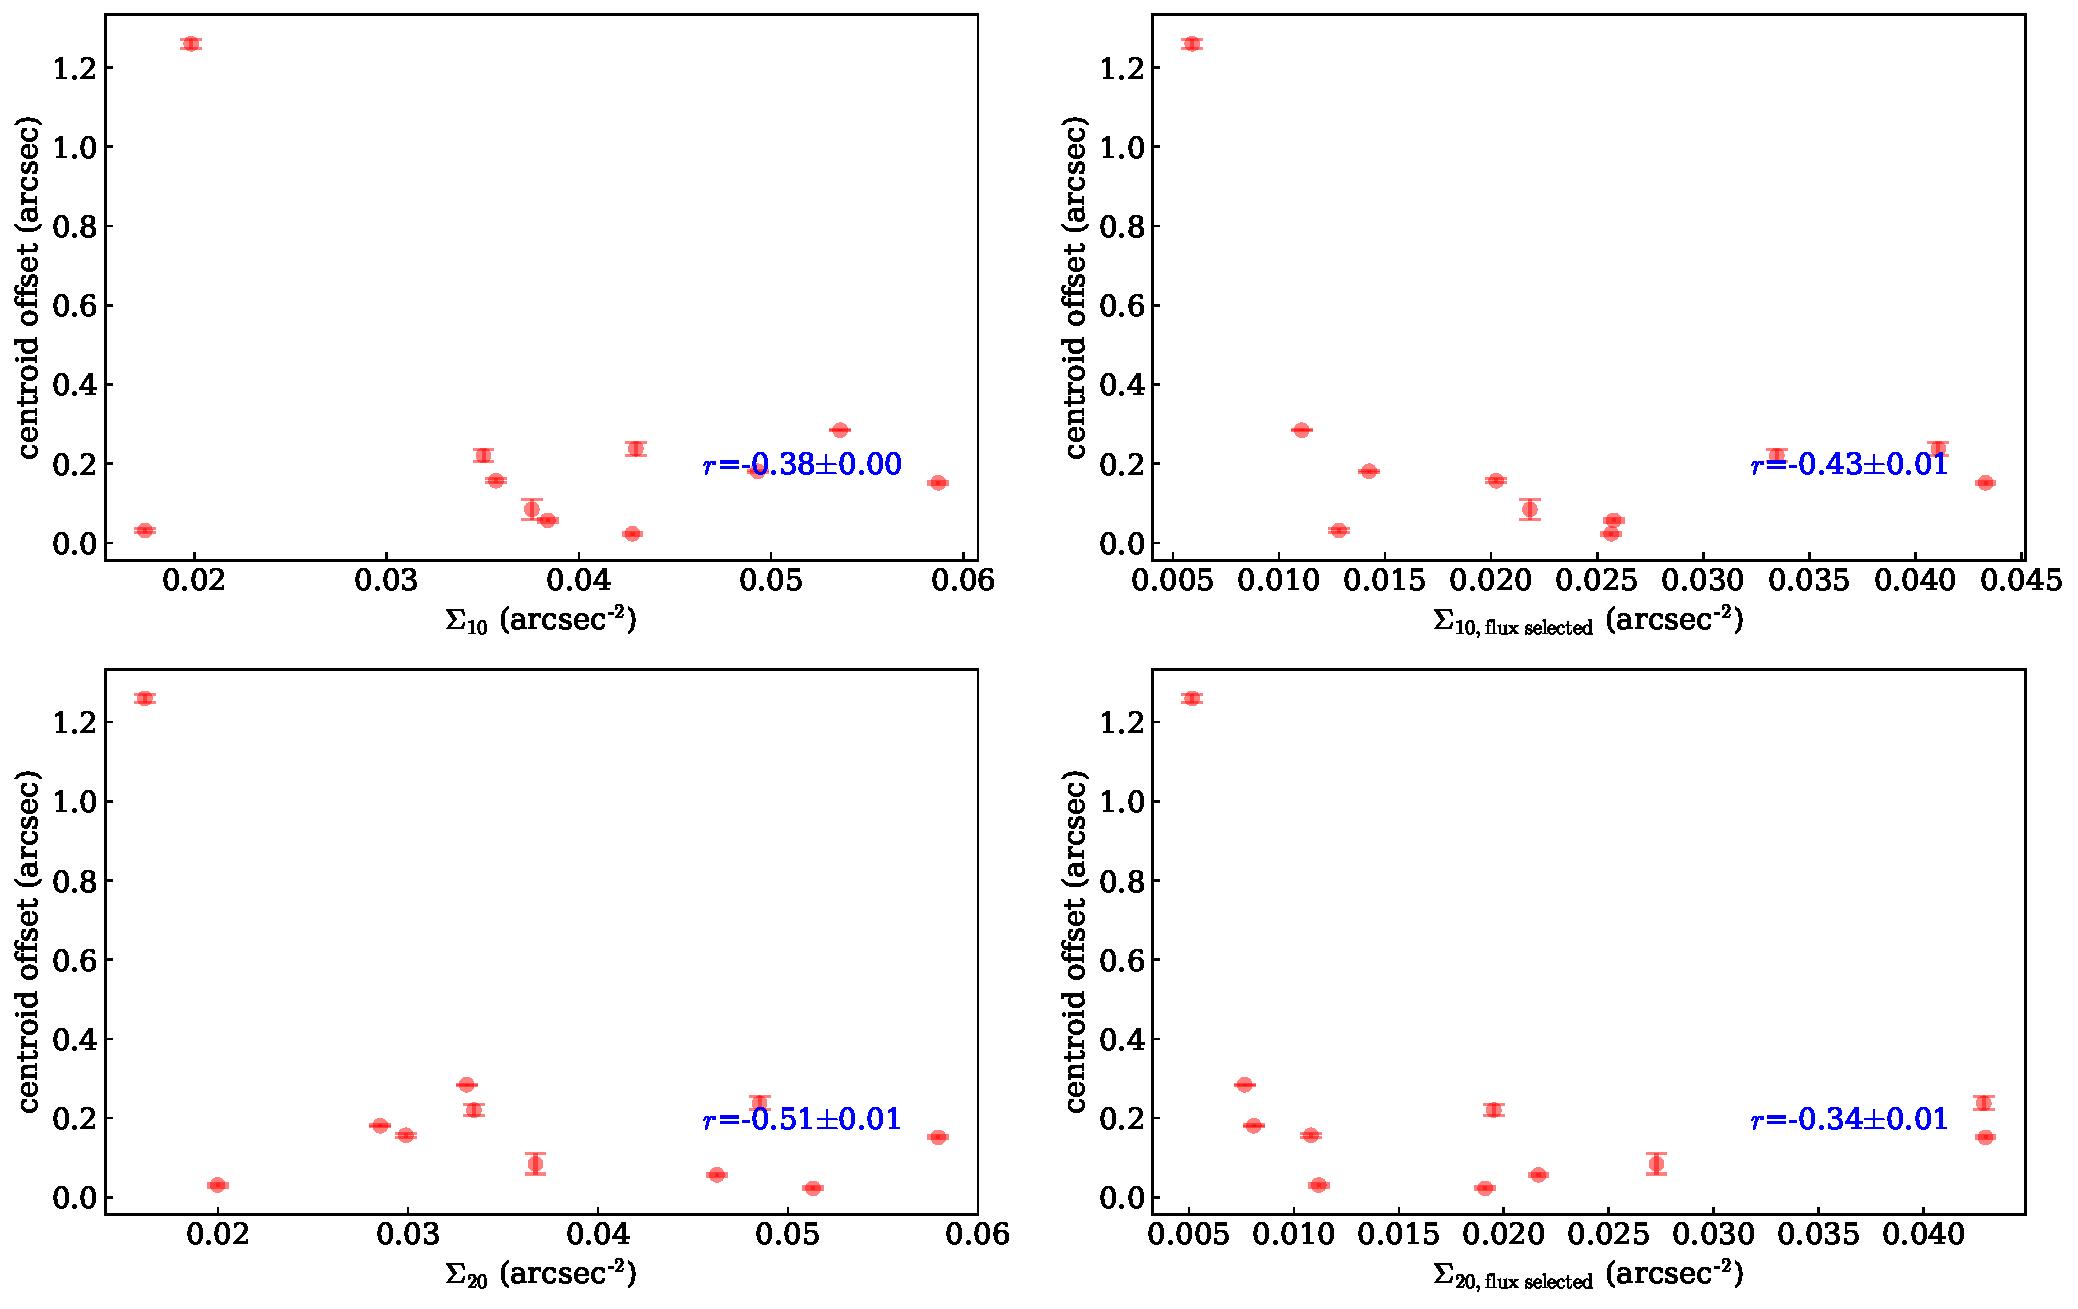
\includegraphics[width=\textwidth]{paper/figures/centroid_offset_vs_Sigma_all.pdf}    \caption{\label{fig:cent_off_Sigma_all}Centroid offset vs. $\Sigma$ values.}
\end{figure*}

\begin{figure*}
    \centering
    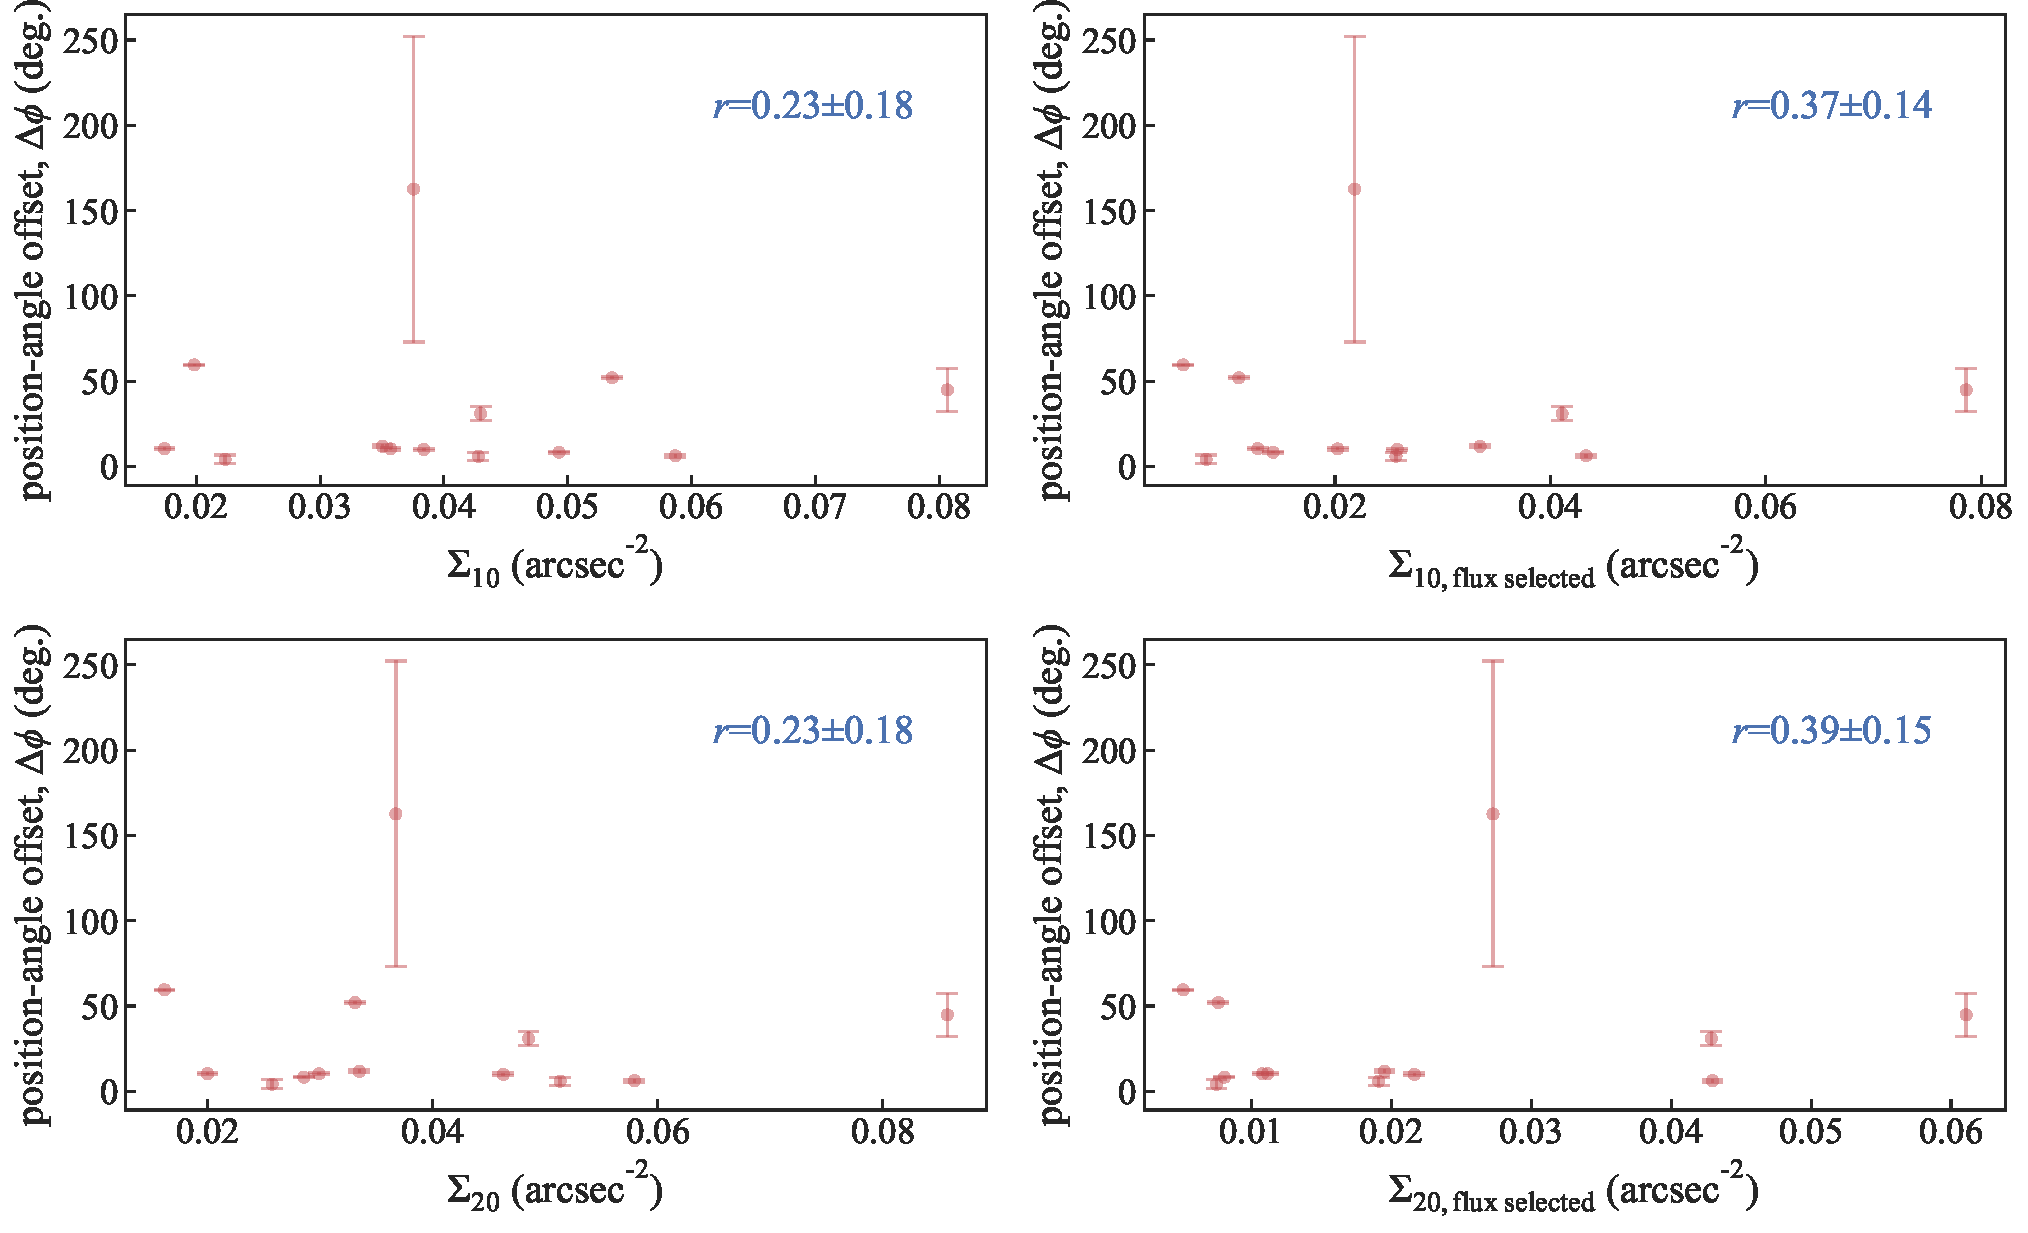
\includegraphics[width=\textwidth]{paper/figures/position_angle_offset_vs_Sigma_all.pdf}
    \caption{\label{fig:pos_off_Sigma_all}Position-angle offset vs. $\Sigma$ values.}
\end{figure*}


% need table of model parameters, example https://arxiv.org/pdf/2008.11724.pdf
\renewcommand{\arraystretch}{1.3}
\begin{table*}
\caption{Lens model profiles: 
\label{table:lens_profiles}
}
\begin{tabular}{cccc}
\hline
System name    & Mass Profiles   & Lens-light profiles      & Source-light profiles    \\ \hline \hline

DESIJ0132-1600 & EPL, Shear      & Double Elliptical S\'ersic & \begin{tabular}[c]{@{}c@{}}Elliptical S\'ersic, \\ Shapelets (n_\text{max} = 10)\end{tabular}     \\ \hline
DESIJ0136-0008 & EPL, SIE, Shear & Double Elliptical S\'ersic & \begin{tabular}[c]{@{}c@{}}Elliptical S\'ersic, \\ Shapelets (n_\text{max} = 10)\end{tabular}      \\ \hline
DESIJ0201-2739 & EPL, SIE, Shear & Double Elliptical S\'ersic & \begin{tabular}[c]{@{}c@{}}Elliptical S\'ersic, \\ Shapelets (n_\text{max} = 8)\end{tabular}           \\ \hline
DESIJ0215-2909 & EPL, Shear      & Double Elliptical S\'ersic & \begin{tabular}[c]{@{}c@{}}Elliptical S\'ersic, \\ Double Shapelets (n_\text{max} = 10)\end{tabular}    \\ \hline
\end{tabular}
\end{table*}

\subsection{Estimation of $\Sigma_{10}$}
In our observations, we assess common environmental factors as outlined in works such as Cooper et al. (2005). Specifically, we determine the galaxy density within a circle whose radius matches the distance to the lens's tenth closest neighboring galaxy, denoted as $\Sigma_{10}$ (as described by Dressler 1980b). Similarly, we compute this density using the twentieth nearest neighbor, labeled $\Sigma_{20}$. We term this environmental measure as the "localized" density.

After background subtraction, we identified sources using the \text{detect\_sources} functionality from our image segmentation approach. To address source overlap, we employed an image deblending method utilizing multiple thresholds, specifically setting the threshold 3 to 5 times the background RMS. Post-identification, certain sources were manually excluded due to their non-adjacency to the primary lensing galaxies. Our calculations encompassed four distinct scenarios: $\Sigma_{10}$, $\Sigma_{10,\text{flux selected}}$, $\Sigma_{20}$, and $\Sigma_{20,\text{flux selected}}$. Notably, in the flux-selected instances, galaxies were filtered based on a $1\%$ flux criterion relative to the central deflecting galaxy.

\subsection{Mass and light alignment}
% Pearson correlation coefficient: https://en.wikipedia.org/wiki/Pearson_correlation_coefficient
In this subsection, we present our results on the alignment between the mass and light distributions in our sample lensing systems.
\subsubsection{Centroid}
There is a weak positive correlation between centroid offset and $\Sigma_{10}$ ($r=0.10$). However, in the case of flux-selected densities,  the correlation becomes negative, with a value of $r= - 0.11$ for $\Sigma_{10, flux selected}$. The correlation between centroid offset and $\Sigma_{20}$ is also negative with a slightly higher coefficient of $r = - 0.27$. For $\Sigma_{20, flux selected}$, the correlation decreases slightly to $r= - 0.18$.

\subsubsection{Position angle}
There is a weak correlation between the misalignment of the position angle ($\Delta \phi$) and $\Sigma_{10}$ ($r=0.23$), which matches the correlation between position angle offset ($\Delta \phi$) and $\Sigma_{20}$ ($r=0.23$). In the flux-selected instances, although the correlation is slightly higher, it remains relatively weak. The correlation between the misalignment of the position angle ($\Delta \phi$) and $\Sigma_{10, flux selected}$ is $r=0.37$, while for $ \Sigma_{20, flux selected}$, the correlation coefficient increases marginally to $r=0.39$.

\section{Discussion and conclusion} \label{sec:discussion}

% conclusion of the paper goes here

% discussion
We discuss our results and conclude by suggesting some arenas of possible future work.

\subsection{Assumptions and results in the context of previous studies}
The main simplifying assumption we make is that the distribution of mass in gravitational lenses is a superposition of elliptical power law and `external shear' which roughly accounts for the effect of neighboring galaxies and cosmic shear. In the two cases of correlation analysis, instead of `external shear', we use the photometric densities considering a certain number of nearest sources. It allows us to estimate the correlations without resorting to the contentious measures of `external shear'.

Considering a mean z $\sim$ 0.5,  the centroid offset of light and mass distribution is within the range of 200 pc predicted by the EAGLE simulation (\cite{Schaller15}). Our sample contains an outlier (J0136-0008) with a centroid offset of $\sim$7.89 kpc. On visual inspection, it appears to be a merger of two galaxies. The analyses are most similar to those of \cite{Treu09} and use similar measures for quantifying source density. Though the correlations are weaker than in some previous studies, the general trend is very similar.

\subsection{Possible future works}
We model the system with a generic flexible model of light and mass which is composed of many more parameters than we were able to analyze in our study. In particular, the mass-density gradient ($\gamma$) encrypts valuable information on the distribution of dark matter. Correlation analyses similar to those performed in \cite{Treu09} or more complex analyses can be done on these values we found. Multiple previous studies such as \cite{Etherington23}, \cite{VandeVyvere22}, \cite{VandeVyvere22b} argue that the profiles used in lensing system modeling are not adequate in terms of complexity and thus the typical combination of EPL with an 'external shear' does not rightly describe the mass distribution of the lensing systems. Especially, the 'external shear' is not the physical shear that it appears to represent; rather, it is a fudge to accommodate for the required flexibility modeling components. In the modeling process, we have estimated the best-fit values of two independent measures of shear($\gamma_\text{shear}$  &  $\phi_\text{shear}$). These values together with photometric source densities can be valuable in the process of finding adequately flexible models of mass distribution.

\begin{acknowledgements}
      Part of this work was supported by the German
      \emph{Deut\-sche For\-schungs\-ge\-mein\-schaft, DFG\/} project
      number Ts~17/2--1.
\end{acknowledgements}

% WARNING
%-------------------------------------------------------------------
% Please note that we have included the references to the file aa.dem in
% order to compile it, but we ask you to:
%
% - use BibTeX with the regular commands:
%   \bibliographystyle{aa} % style aa.bst
%   \bibliography{Yourfile} % your references Yourfile.bib
%
% - join the .bib files when you upload your source files
%-------------------------------------------------------------------

% - use BibTeX with the regular commands:
\bibliographystyle{aa} % style aa.bst
\bibliography{ajshajib} % your references Yourfile.bib

\appendix

\section{[For extra figures]}

\end{document}